\documentclass[a4paper]{article}
\usepackage[utf8]{inputenc}
\usepackage[english]{babel}
\usepackage{pdfpages, titling}
\usepackage{array, float, arydshln}
\usepackage{cite, tablefootnote}
\usepackage{graphicx, caption}
\usepackage{listings}
\usepackage{color}
\usepackage{mathtools, braket}
\usepackage{amssymb}
\usepackage[nottoc]{tocbibind} % references in the toc
\usepackage{subcaption}
\usepackage{textcomp}
\usepackage{minted}
\usepackage[hidelinks]{hyperref}
\graphicspath{{Pictures/}} % Specifies the directory where pictures are stored

\newcommand{\vect}[1]{\boldsymbol{#1}}
\newcommand{\subtitle}[1]{
  \posttitle{
    \par\end{center}
    \begin{center}\large#1\end{center}
    \vskip0.5em}
}
\lstset{frame=tb,
  language=Java,
  aboveskip=3mm,
  belowskip=3mm,
  showstringspaces=false,
  columns=flexible,
  basicstyle={\small\ttfamily},
  numbers=none,
  breaklines=true,
  breakatwhitespace=true,
  tabsize=3
}

\author{Jaro Camphuijsen (6042473) and Rahiel Kasim (10447539)}
\title{Scientific Computing III}
\subtitle{SciCoPyth Waving Goodbye!}

\begin{document}
\maketitle

\tableofcontents

\section{Eigenmodes of drums or membranes of different shapes}
\subsection{Theory}
When we want to find the eigenmodes of a vibrating surface, we want to solve the two dimensional wave equation and find a seperable solution:
\begin{equation}
\frac{1}{T(t)}\frac{\partial ^2 T(t)}{\partial t^2} = c^2 \frac{1}{v(x,y)} \nabla ^2 v(x,y)
\label{eq:wave2d}
\end{equation}

Because we are interested in the time independent eigenmodes we want to solve only the right hand side of equation \ref{eq:wave2d} where we can replace the left hand side by a constant K.\footnote{Both the left and right hand side of equation \ref{eq:wave2d} are constant since one depends on only t and one on only x and y. This is the separable behaviour of the solution we are looking for.} We end up with the following equation:

\begin{equation}
\nabla ^2 v(x,y) = K v(x,y)
\label{eq:wavexy}
\end{equation}

Which we can discretize:

\begin{equation}
\frac{v_{i+1,j} - 2v_{i,j} + v_{i-1,j}}{\Delta x^2} + \frac{v_{i,j+1} - 2v_{i,j} + v_{i,j-1}}{\Delta y^2} =
K v_{i,j}
\label{eq:waveDiscr}
\end{equation}

By setting $\Delta x = \Delta y = \sqrt{\lambda / K}$ and we can simplify this to:
\begin{equation}
 v_{i+1,j} + v_{i,j+1} + v_{i-1,j} + v_{i,j-1} - 4v_{i,j} = \lambda v_{i,j}
\label{eq:waveDiscrSimp}
\end{equation}

We can write this out explicitly for a $2\times2$ system and construct the equations in matrix form. All boundaries are set to zero so we can drop all terms with $i$ or $j = 0$ or $3$ in the matrix equation:

\begin{equation}
\begin{aligned}
v_{2,1} + v_{1,2} + v_{0,1} + v_{1,0} - 4v_{1,1} =  \lambda v_{1,1} \\
v_{3,1} + v_{2,2} + v_{1,1} + v_{2,0} - 4v_{2,1} =  \lambda v_{2,1} \\
v_{2,2} + v_{1,3} + v_{0,2} + v_{1,1} - 4v_{1,2} =  \lambda v_{1,2}\\
v_{3,2} + v_{2,3} + v_{1,2} + v_{2,1} - 4v_{2,2} =  \lambda v_{2,2}
\end{aligned}
\label{eq:waveDiscrExpl}
\end{equation}



\begin{equation}
\begin{bmatrix*}[r]
    -4 & 1 & 1 & 0 \\
    1 & -4 & 0 & 1 \\
    1 & 0 & -4 & 1 \\
    0 & 1 & 1 & -4
\end{bmatrix*}
\begin{bmatrix*}
    v_{1,1}\\
    v_{2,1}\\
    v_{1,2}\\
    v_{2,2}
\end{bmatrix*}
=
\lambda
\begin{bmatrix*}
     v_{1,1}\\
    v_{2,1}\\
    v_{1,2}\\
    v_{2,2}
\end{bmatrix*}
\label{eq:mat2x2}
\end{equation}
Equation \ref{eq:mat2x2} is a so called eigenvalue problem, it states that for certain vectors $v_{i,j}$ multiplied by the finite difference matrix, we obtain a scalar multiple of this same vector $\lambda v_{i,j}$. These vectors and scalar factors are called eigenvectors and eigenvalues of the matrix respectively. An eigenvalue problem can be solved directly using the appropriate methods. The eigenvectors represent the possible standing waves in the domain and their eigenvalues give us the frequency of such a wave. 
 
\begin{figure}
\begin{centering}
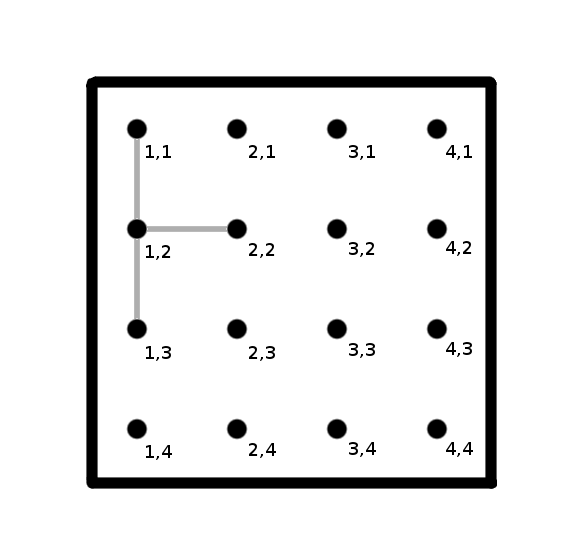
\includegraphics[width=8cm]{stencil.png}
\caption{The stencil for a $4\times4$ system with all connection for the point $(1,2)$.}
\label{fig:stencil4x4}
\end{centering}
\end{figure}

In figure \ref{fig:stencil4x4} we see the stencil for a $4\times4$ system. The connections of point $(1,2)$ are the points $(1,1)$, $(2,2)$, $(1,3)$ and the boundary point $(0,2)$. However since all boundaries are zero we can drop this last point. The matrix representation  of the eigenvalue problem of a square system of arbitrary size can be found in equation \ref{eq:mat4x4} in appendix \ref{app:A}. The connections of point $(1,2)$ in figure \ref{fig:stencil4x4} correspond to the second column of this matrix. 

The solution to the timedependent part in equation \ref{eq:wave2d} where we replace the right hand side by the same constant K, is given by equation \ref{eq:timedepsol}.

\begin{equation}
T(t) = A\sin{c\lambda t} + B\cos{c\lambda t}
\label{eq:timedepsol}
\end{equation}


\subsection{Implementation}
For a square domain with sides n cells, the finite difference matrix grows with $n^4$. As we can see the bigger the system the more zero valued entries we have in our finite difference matrix. When implementing this problem it is not very efficient to store the full matrix but we can use some other format instead. The SciPy library \cite{scipy} offers some useful matrix formats in its \mintinline{python}{sparse} module which store only the nonzero values. This type of matrix saves memory space and iteration loops since we now only have approximately $5L$ entries. 

We also want to find the eigenvalues for different domain shapes. For a circular domain we set all rows and columns corresponding with points outside a certain radius from the domain center to zero. The same is done for a rectangular domain, this time using a domain length of $2L$ so the short side of the rectangle is of length $L$. 

Once found, the eigenmodes can be sorted by their eigenvalue, we also want to ignore all modes with eigenvalue equal to zero since these are not interesting to us because there is no wave in that case.

Once the eigenmodes are found we can evolve them in time using the simple solution of the time dependent part of the wave equation given by equation \ref{eq:timedepsol}. Here we set A to zero so the sine part is discarded and we are only left with the cosine part, we do not lose generality here since we only set the previously found steady state to be amplitude of the wave. 


\subsection{Results}
In figure \ref{fig:eigenmodes_s}, \ref{fig:eigenmodes_r} and \ref{fig:eigenmodes_c} we can see some of the first eigenmodes for these systems. 

\begin{figure}
\centering
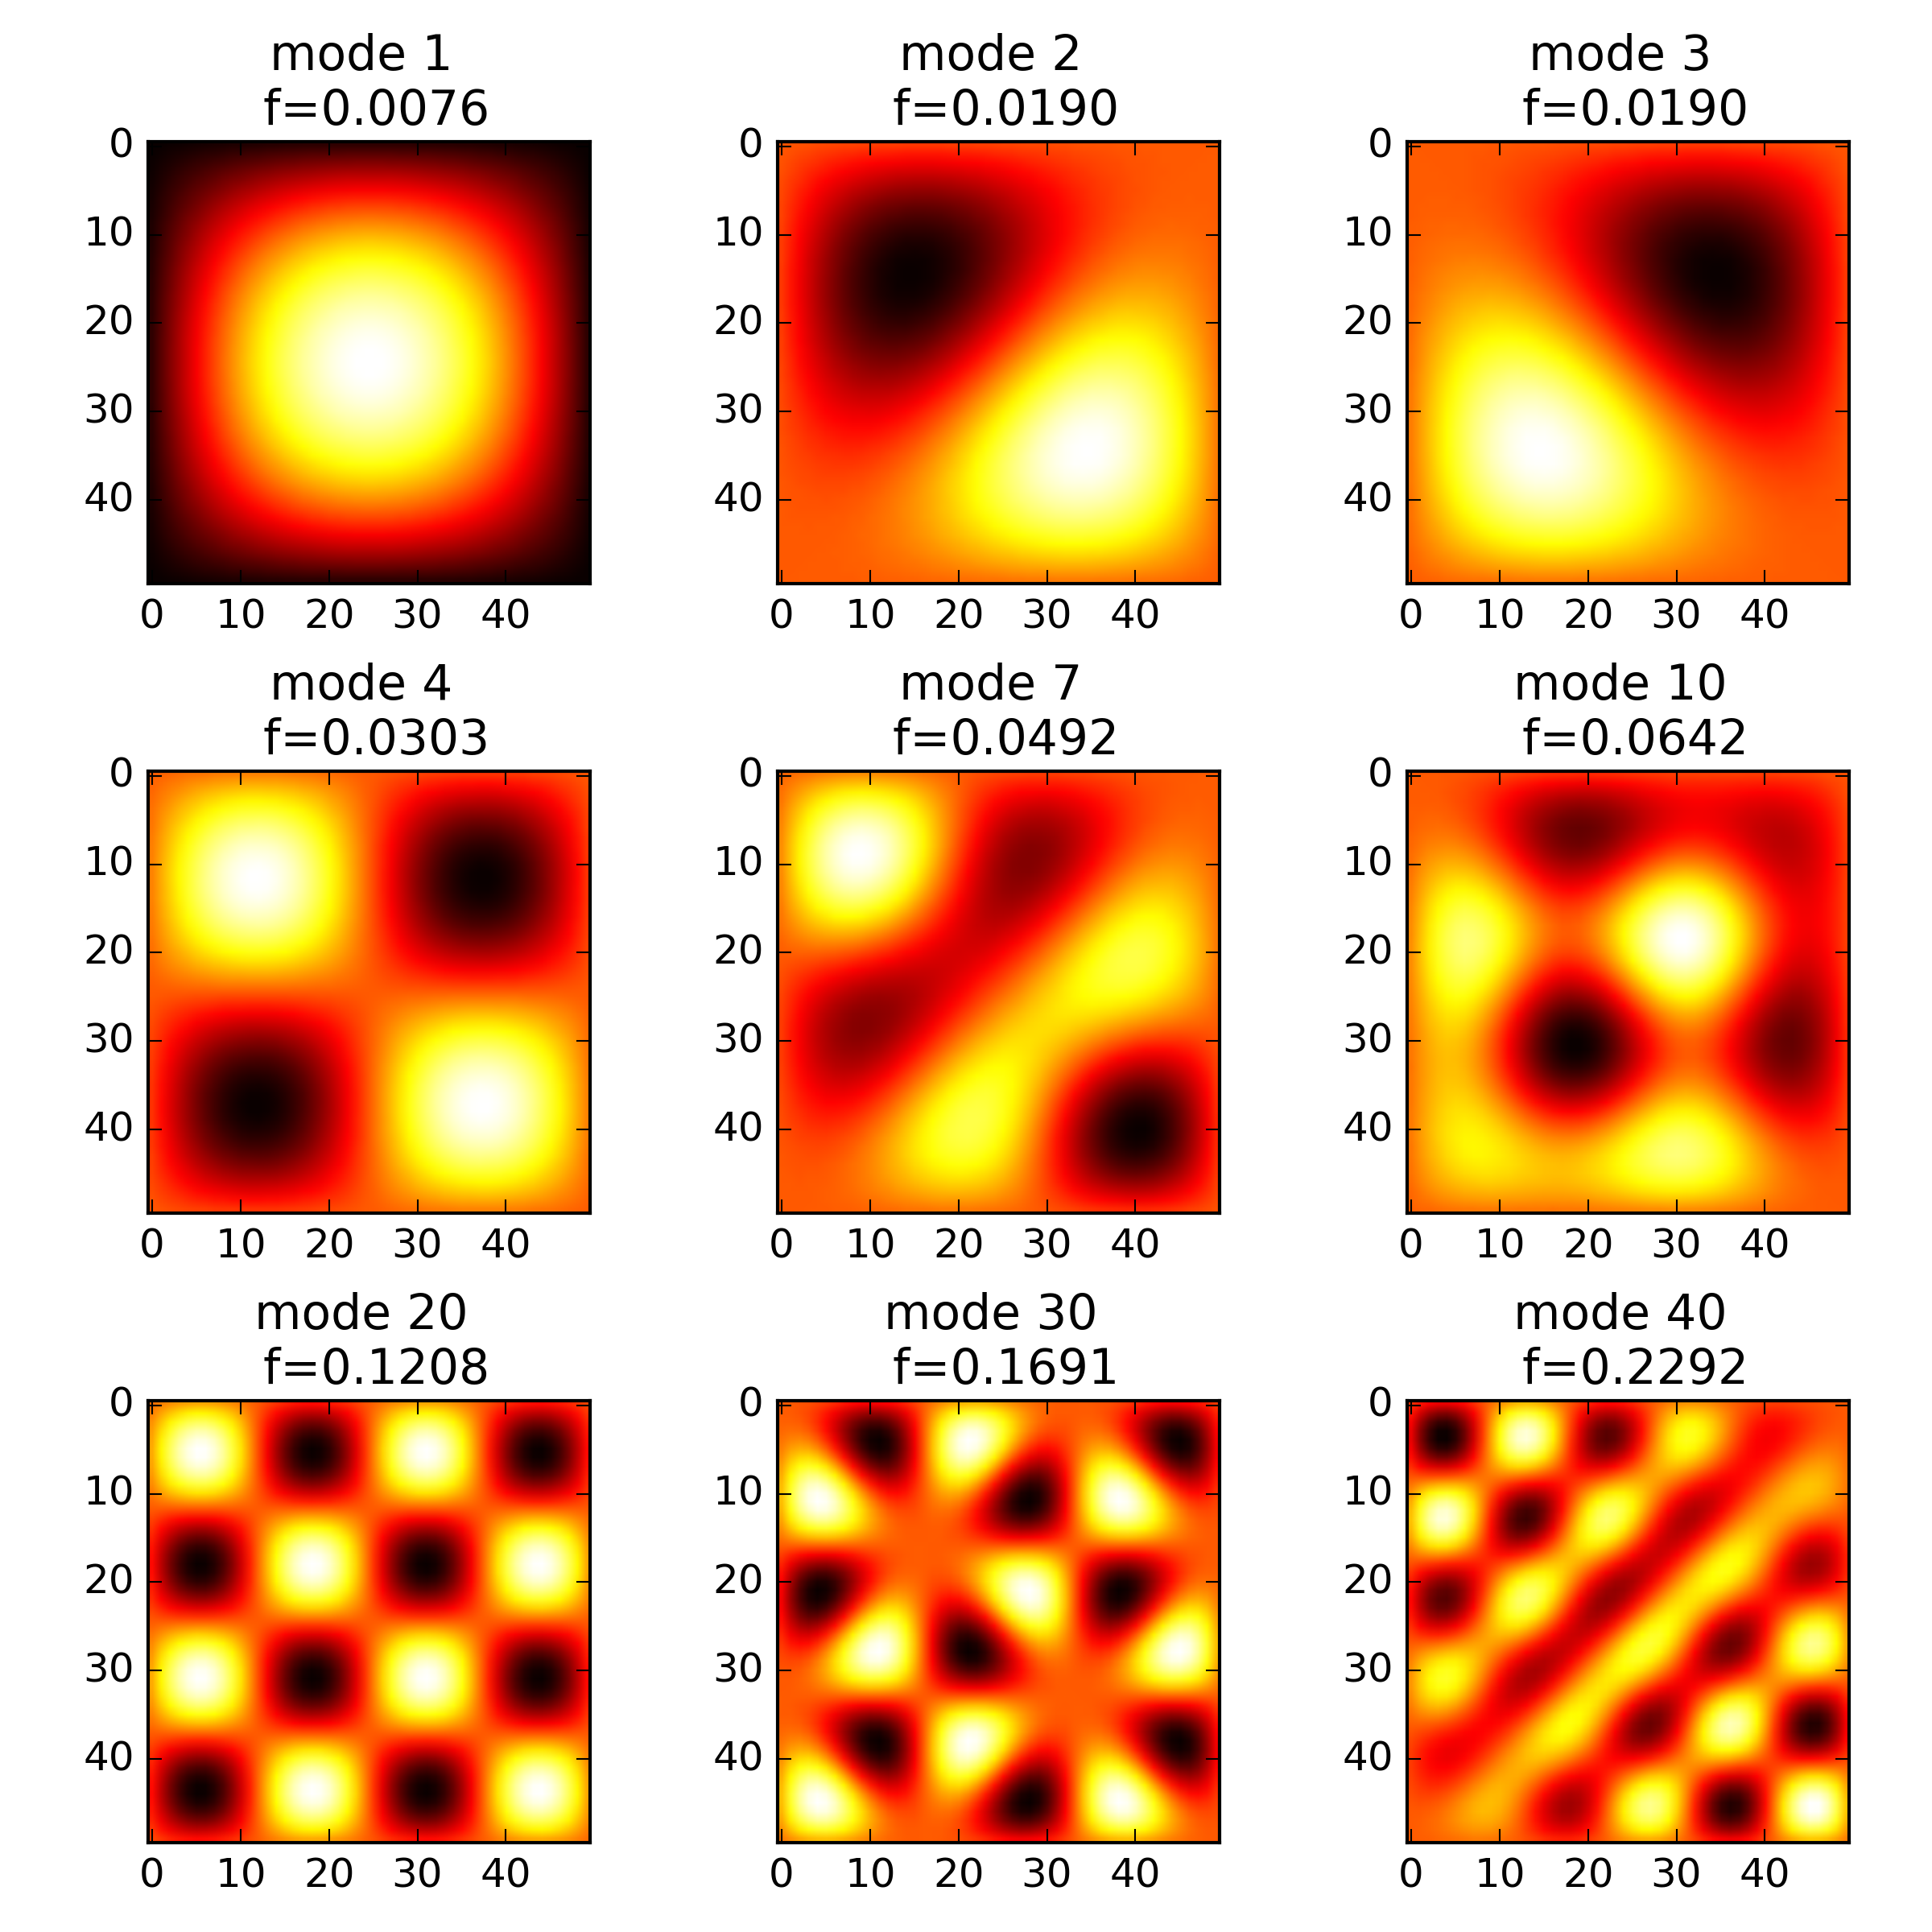
\includegraphics[width=10cm]{Pictures/eigenmodes_s.png}
\caption{Some of the first eigenmodes calculated for a square domain sorted by their frequencies.}
\label{fig:eigenmodes_s}
\end{figure}

\begin{figure}
\centering
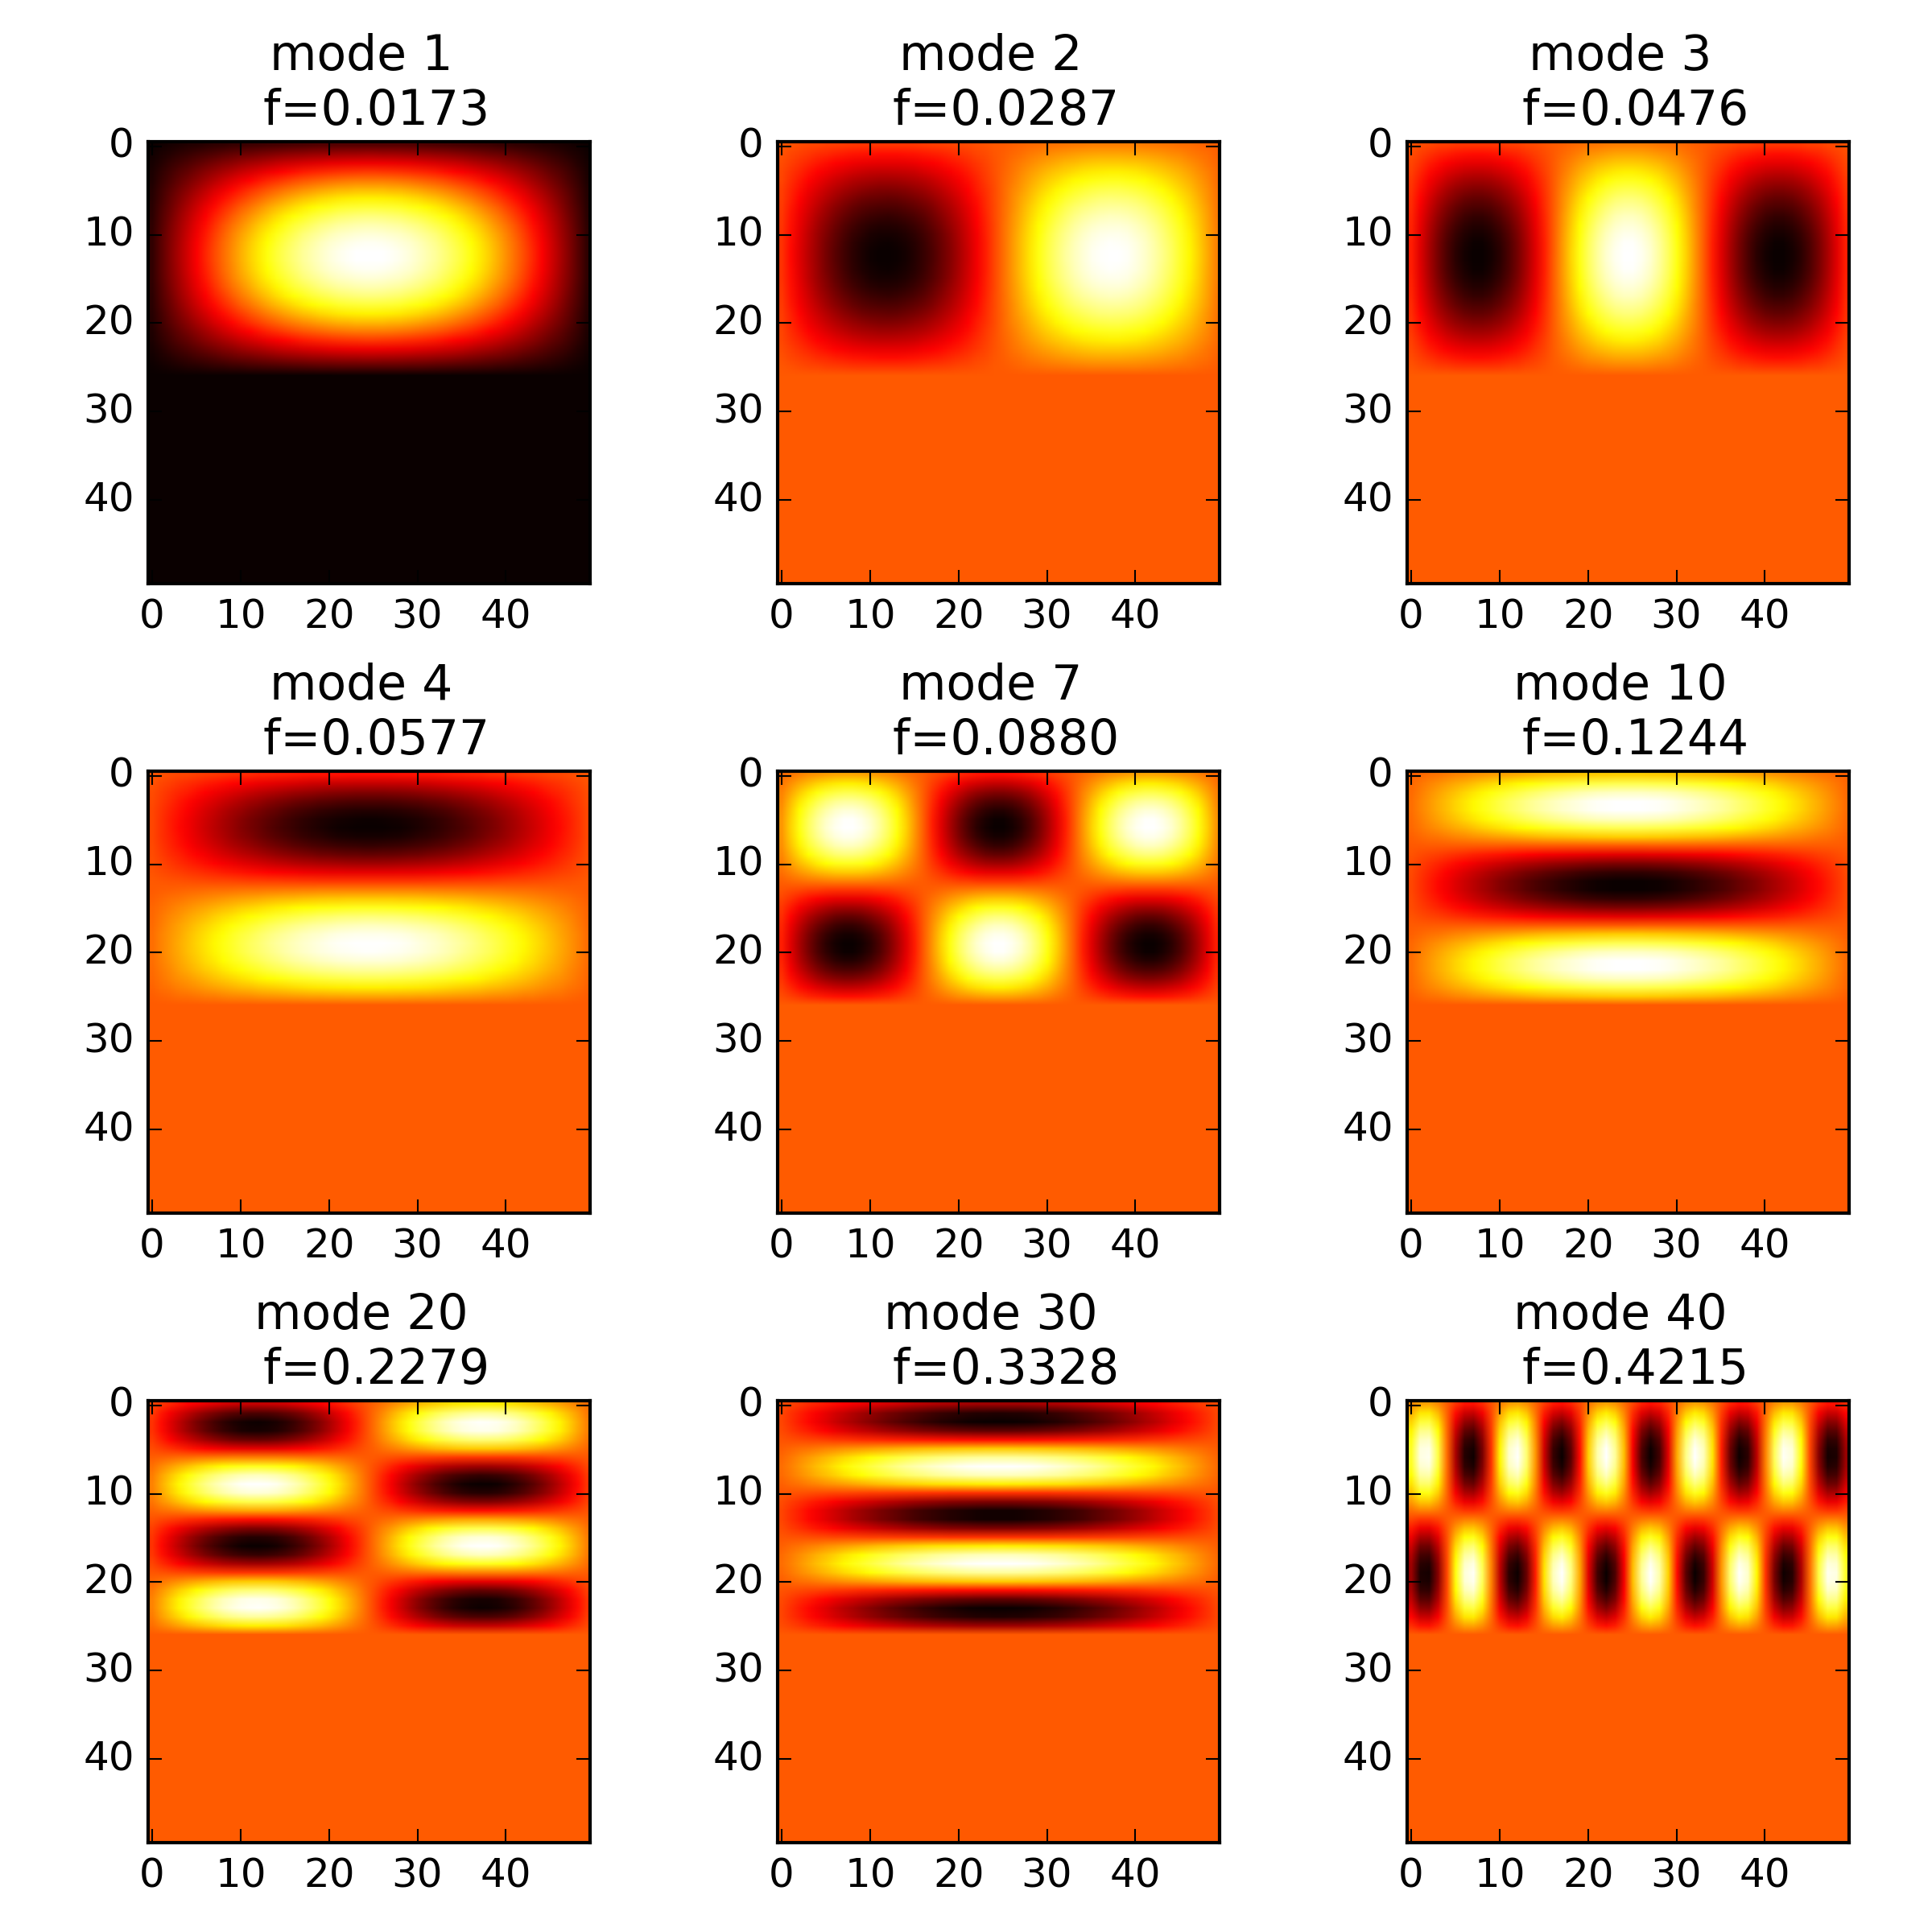
\includegraphics[width=9cm]{Pictures/eigenmodes_r.png}
\caption{Some of the first eigenmodes calculated for a rectangular domain sorted by their frequencies.}
\label{fig:eigenmodes_r}
\end{figure}

\begin{figure}
\centering
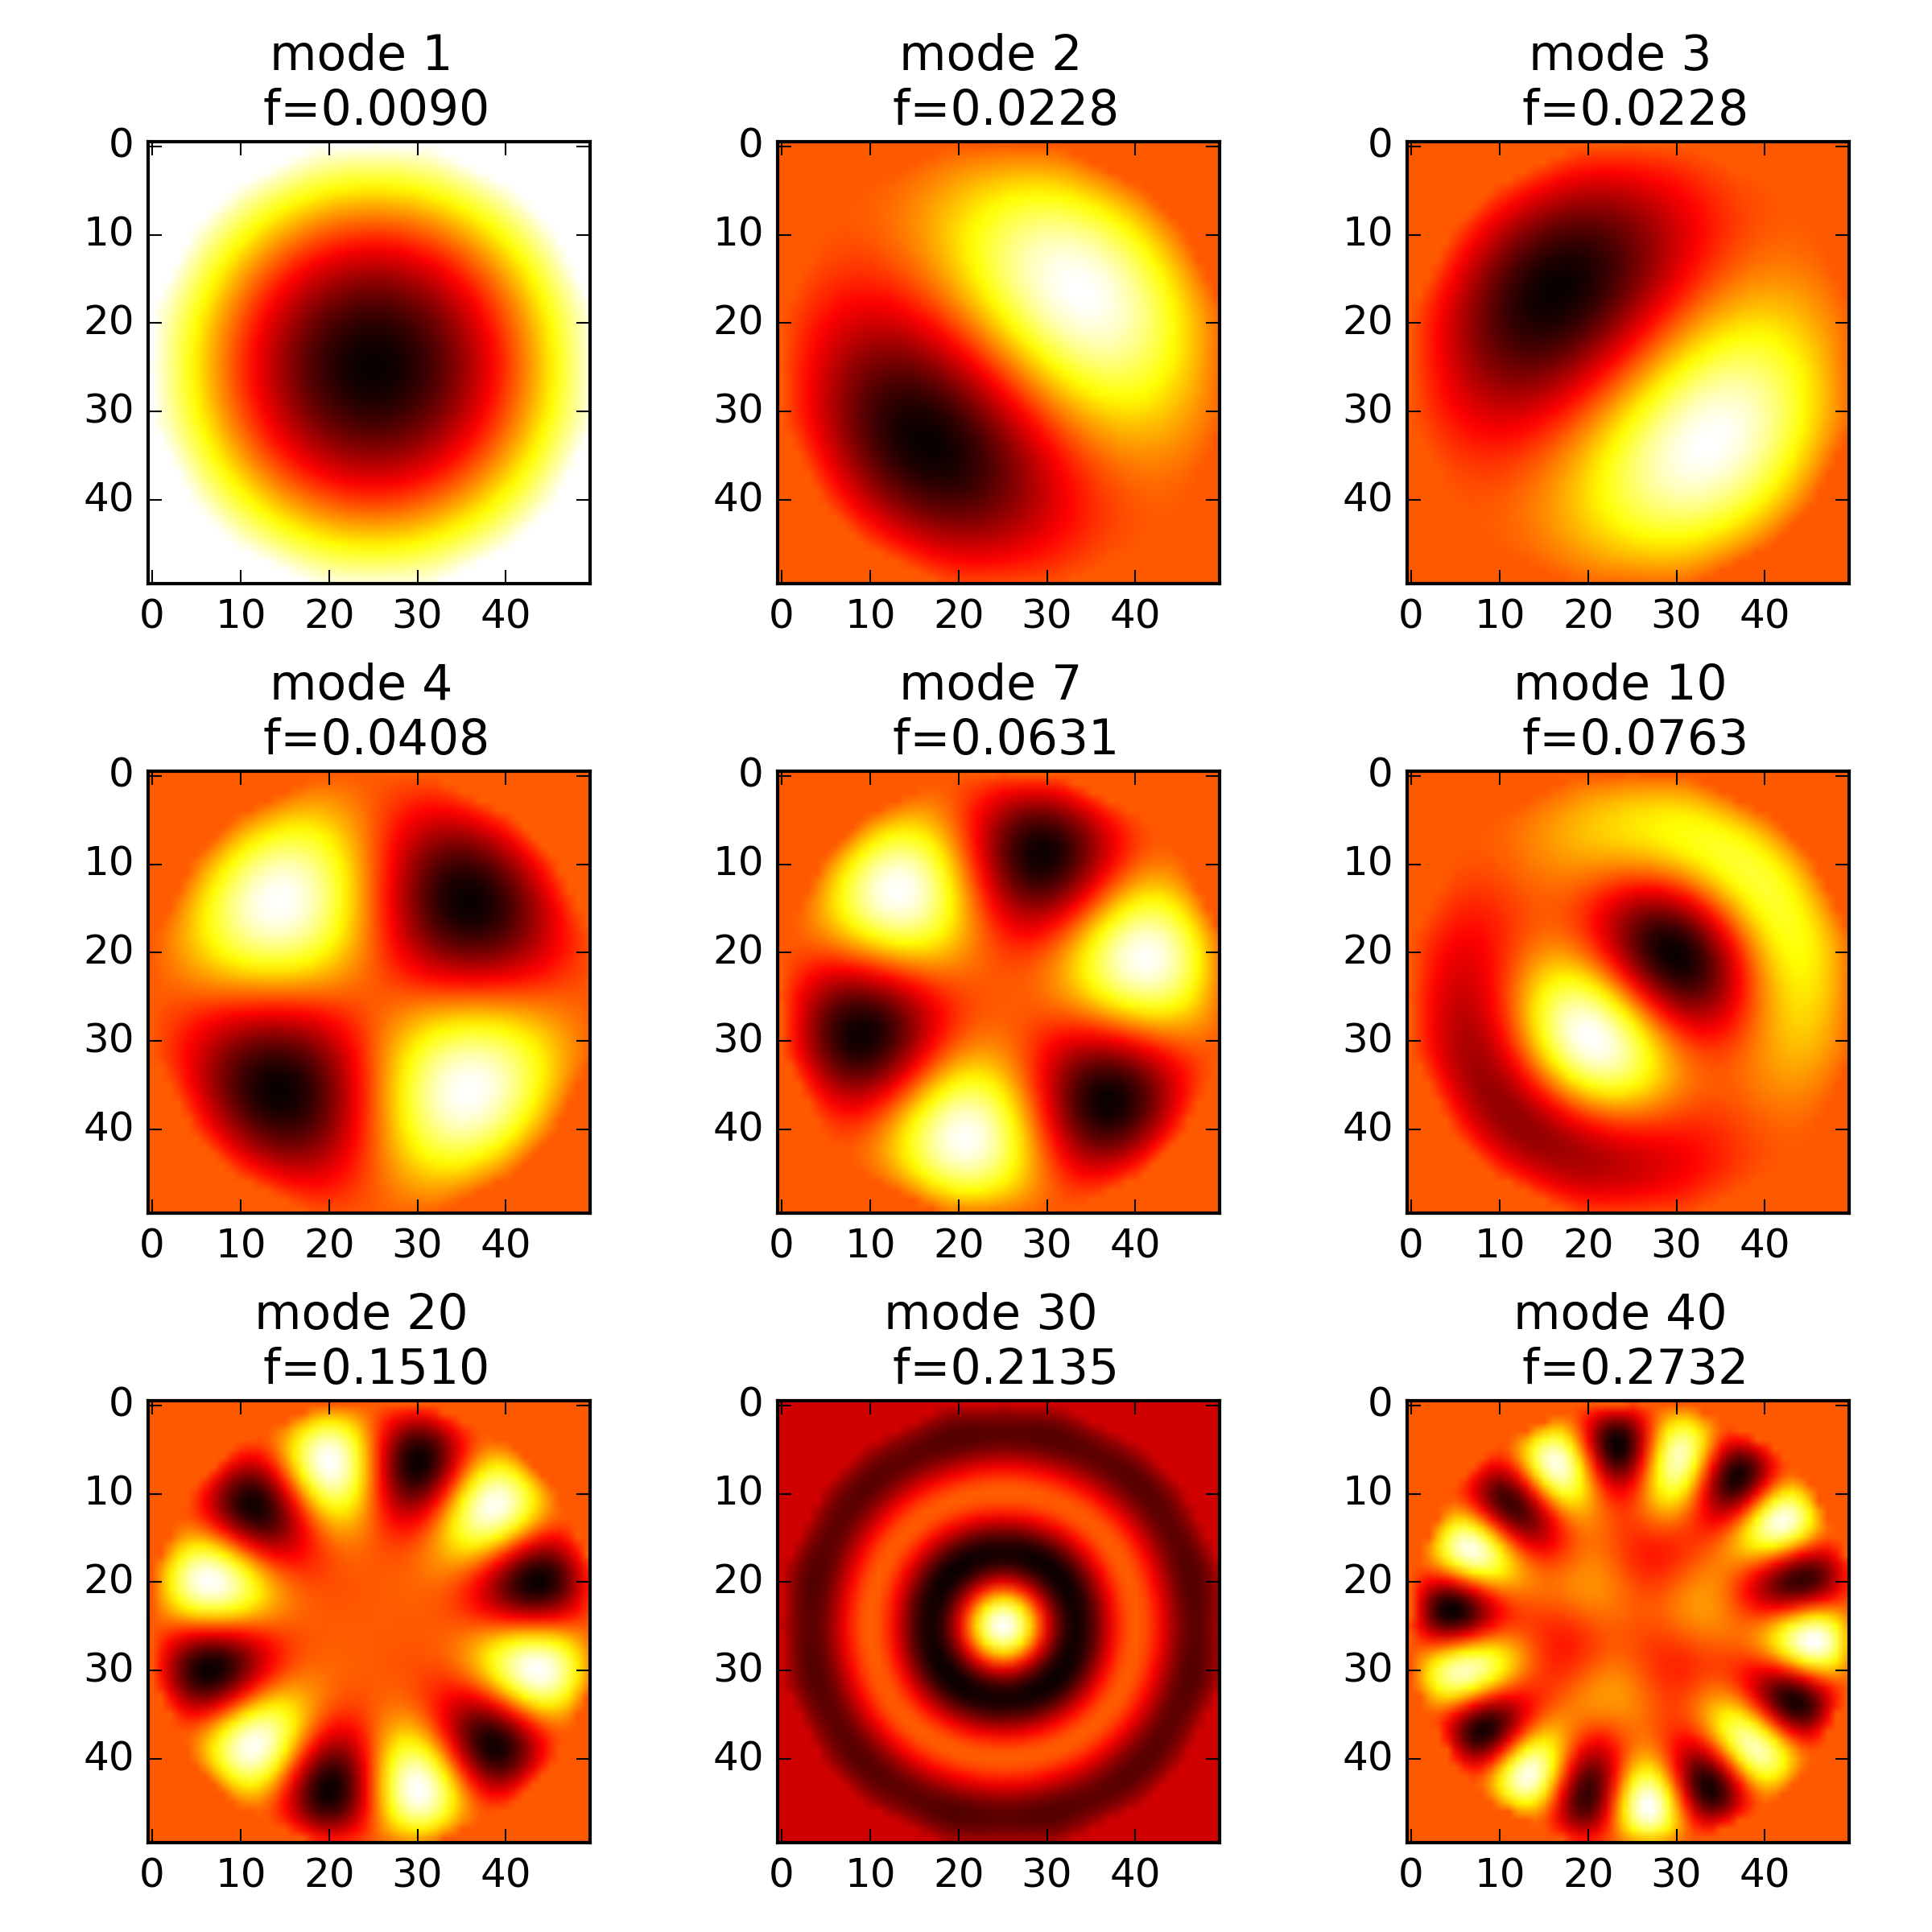
\includegraphics[width=9cm]{Pictures/eigenmodes_c.png}
\caption{Some of the first eigenmodes calculated for a circular domain sorted by their frequencies.}
\label{fig:eigenmodes_c}
\end{figure}

In figure \ref{fig:L_dependence} we see how the eigenfrequencies depend on the size of the domain. We see it corresponds to a $\frac{1}{L^2}$ dependence, which makes sense since our domain area is of size $L^2$.

\begin{figure}
\centering
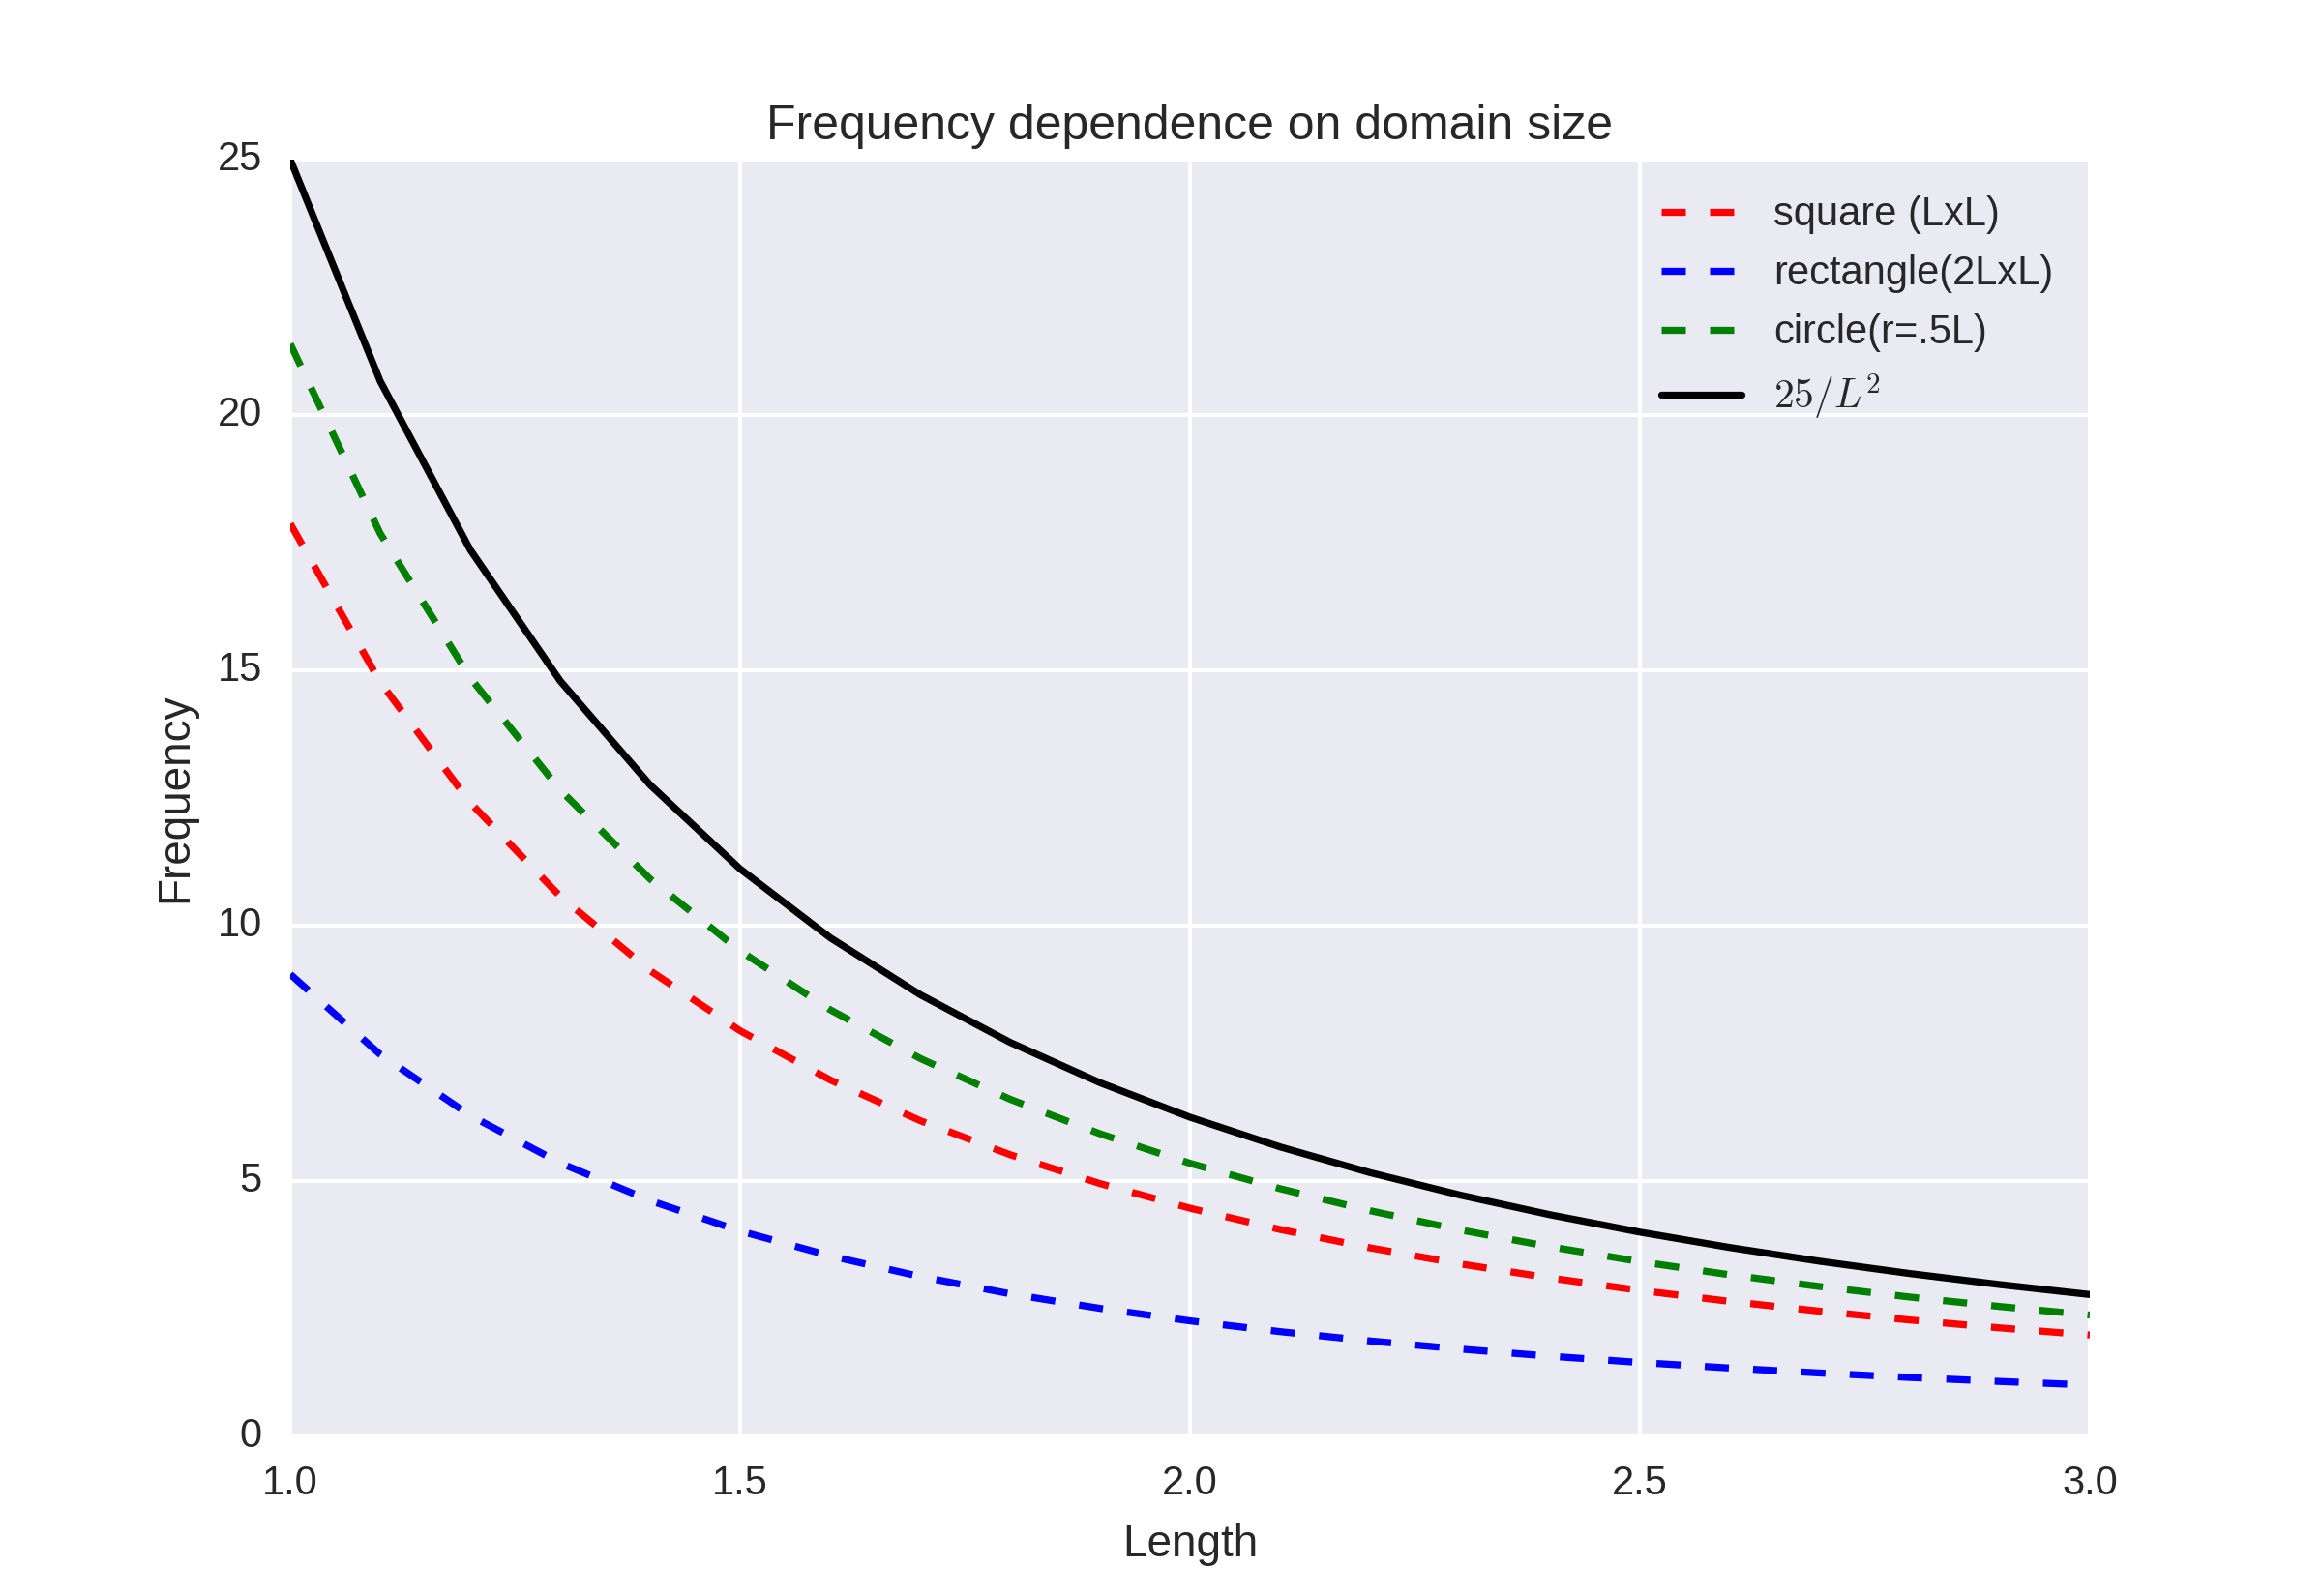
\includegraphics[width=10cm]{Pictures/L_dependence.png}
\caption{Dependence of the eigenfrequency on the size of the domain for three different shapes. A reference line is plotted to show the  $1/L^2$ dependency.}
\label{fig:L_dependence}
\end{figure}

In figure \ref{fig:dstep_dependence} we plotted the relation between 
the number of integration steps and the eigenfrequency. In theory this should not be of any influence since the system itself does not change, however due to limited resolution at low step numbers we get a numerical error in the eigenvalue. We see how the calculated eigenfrequency forms an assymptote which we can assume to be the true eigenfrequency of the system. 

\begin{figure}
\centering
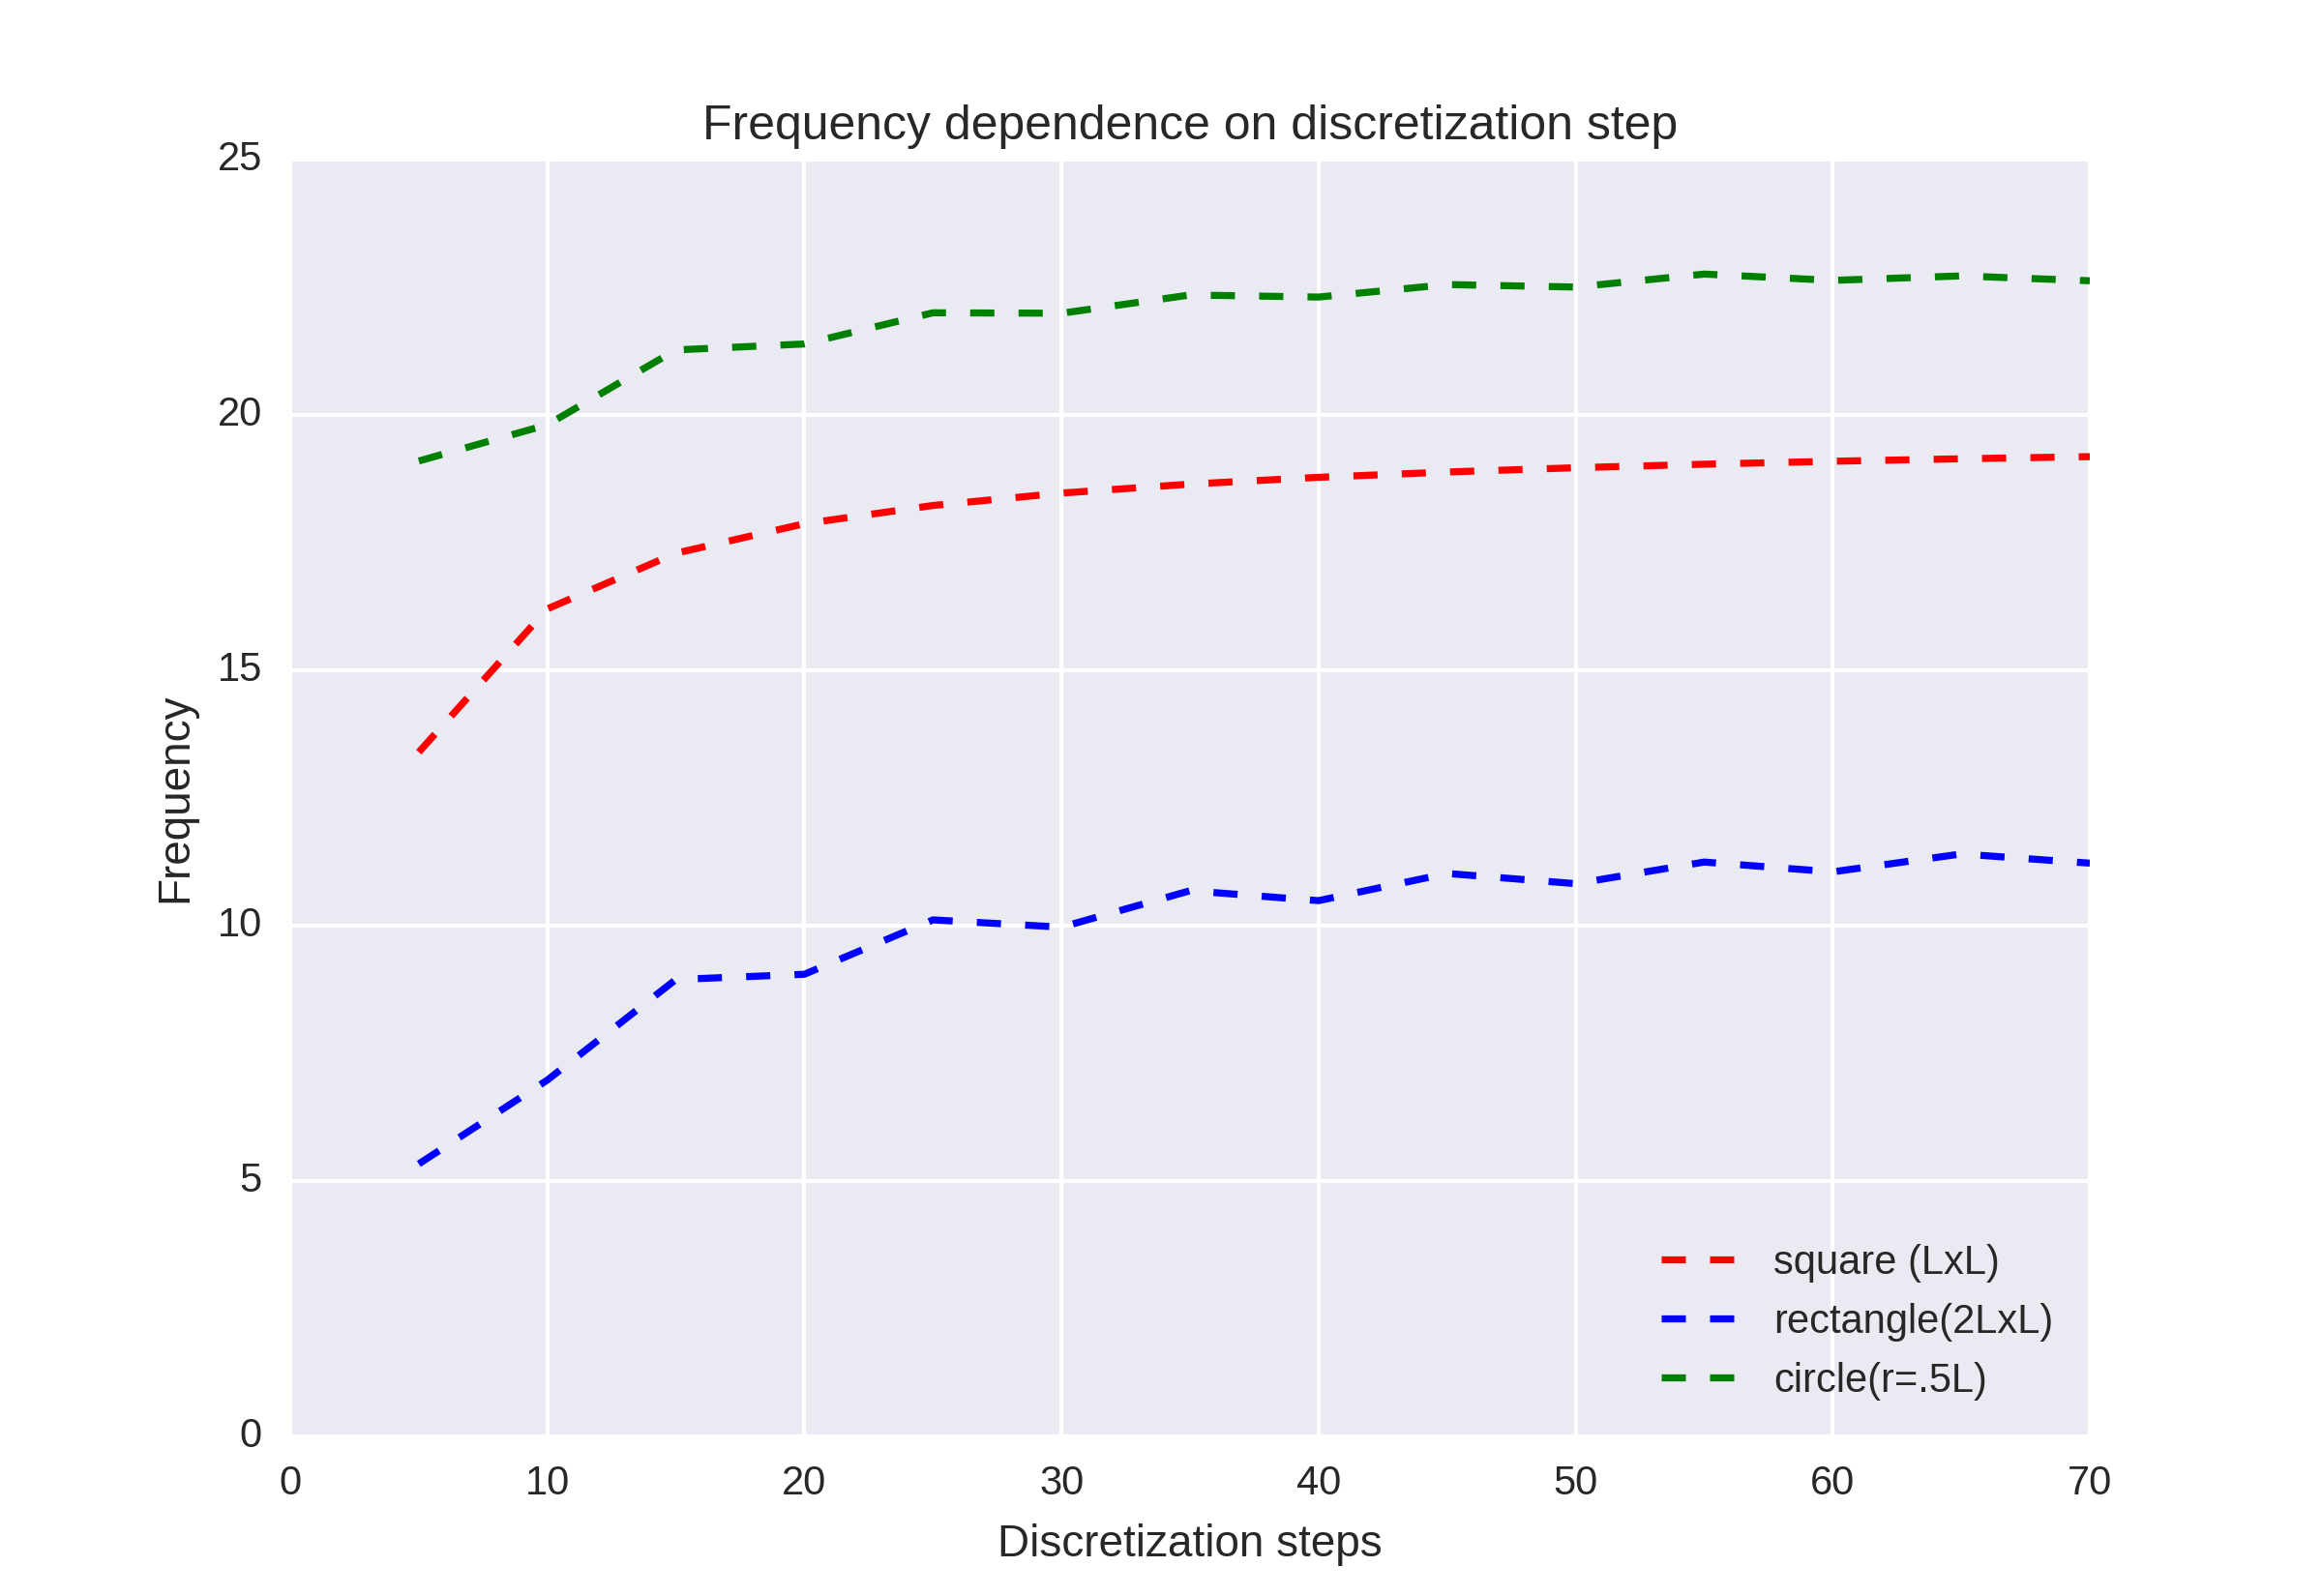
\includegraphics[width=10cm]{Pictures/dstep_dependence.png}
\caption{Dependence of the eigenfrequency on the number of discretization steps}
\label{fig:dstep_dependence}
\end{figure}

The time evolution calculated by equation \ref{eq:timedepsol} is shown in figure \ref{fig:time_evolution_s}, \ref{fig:time_evolution_r} and \ref{fig:time_evolution_c} for different eigenmodes and several timesteps. 

\begin{figure}
\centering
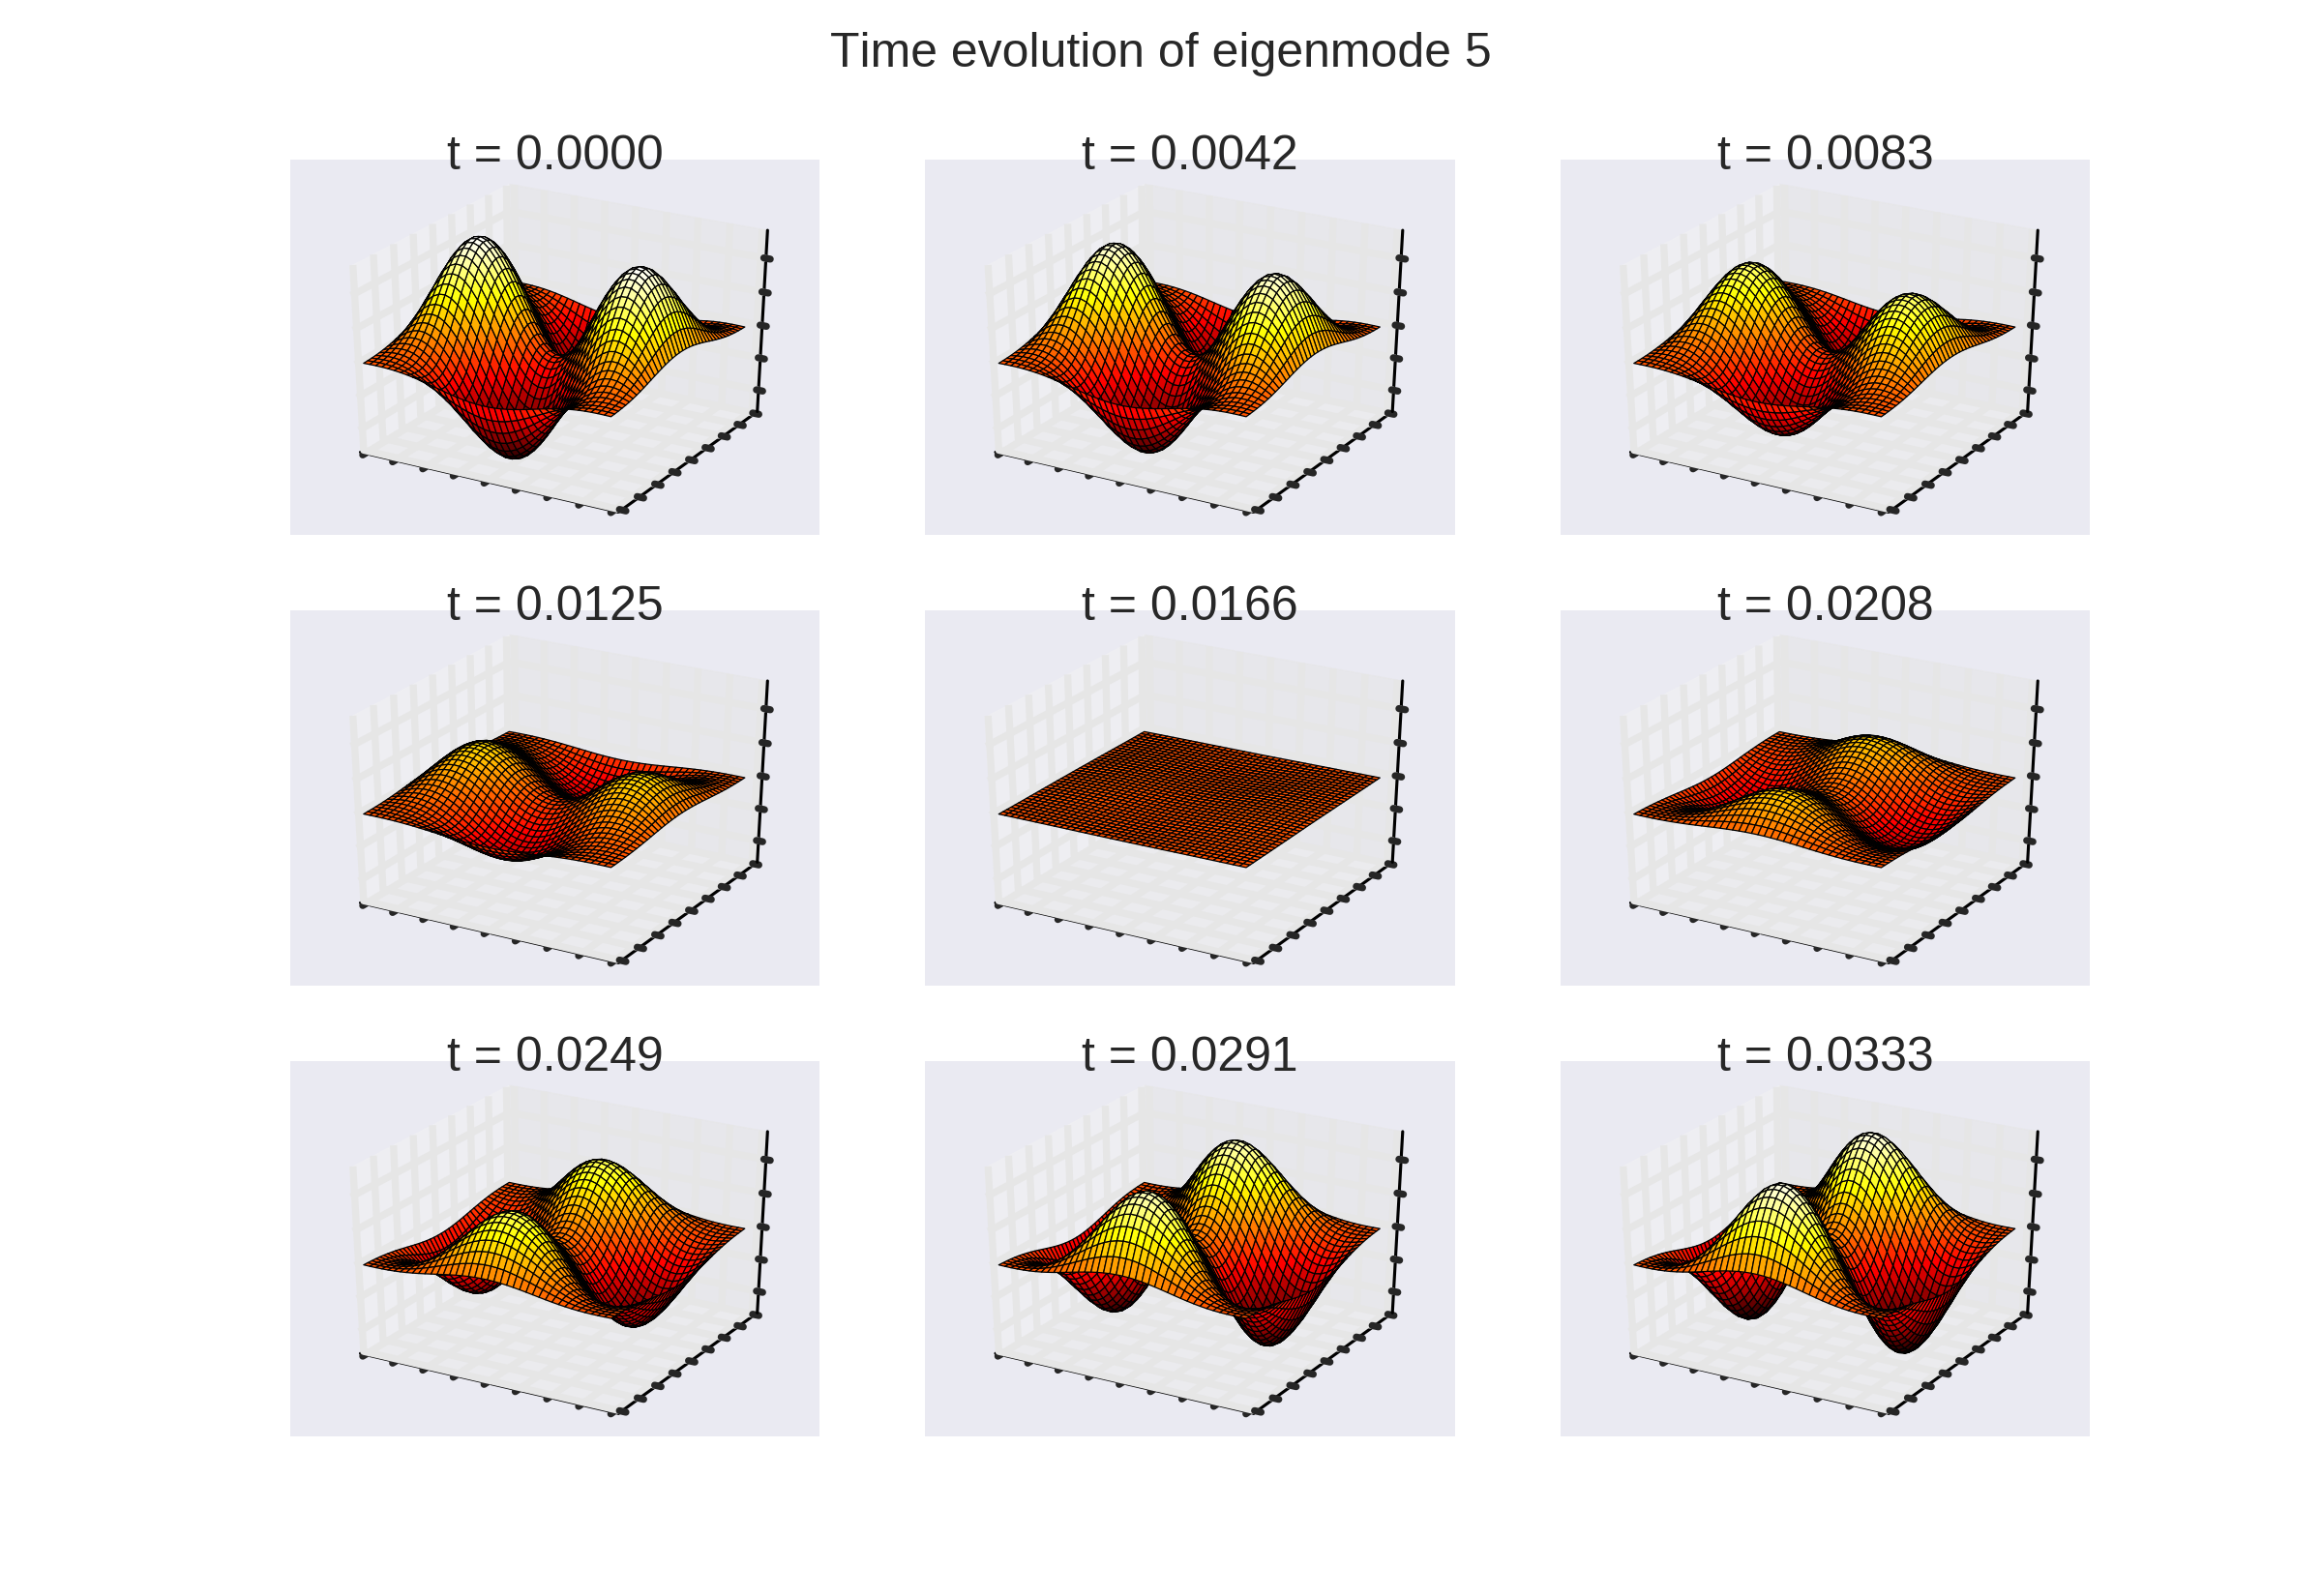
\includegraphics[width=10cm]{Pictures/time_evolution_s.png}
\caption{Some of the first time evolution calculated for a square domain sorted by their frequencies.}
\label{fig:time_evolution_s}
\end{figure}

\begin{figure}
\centering
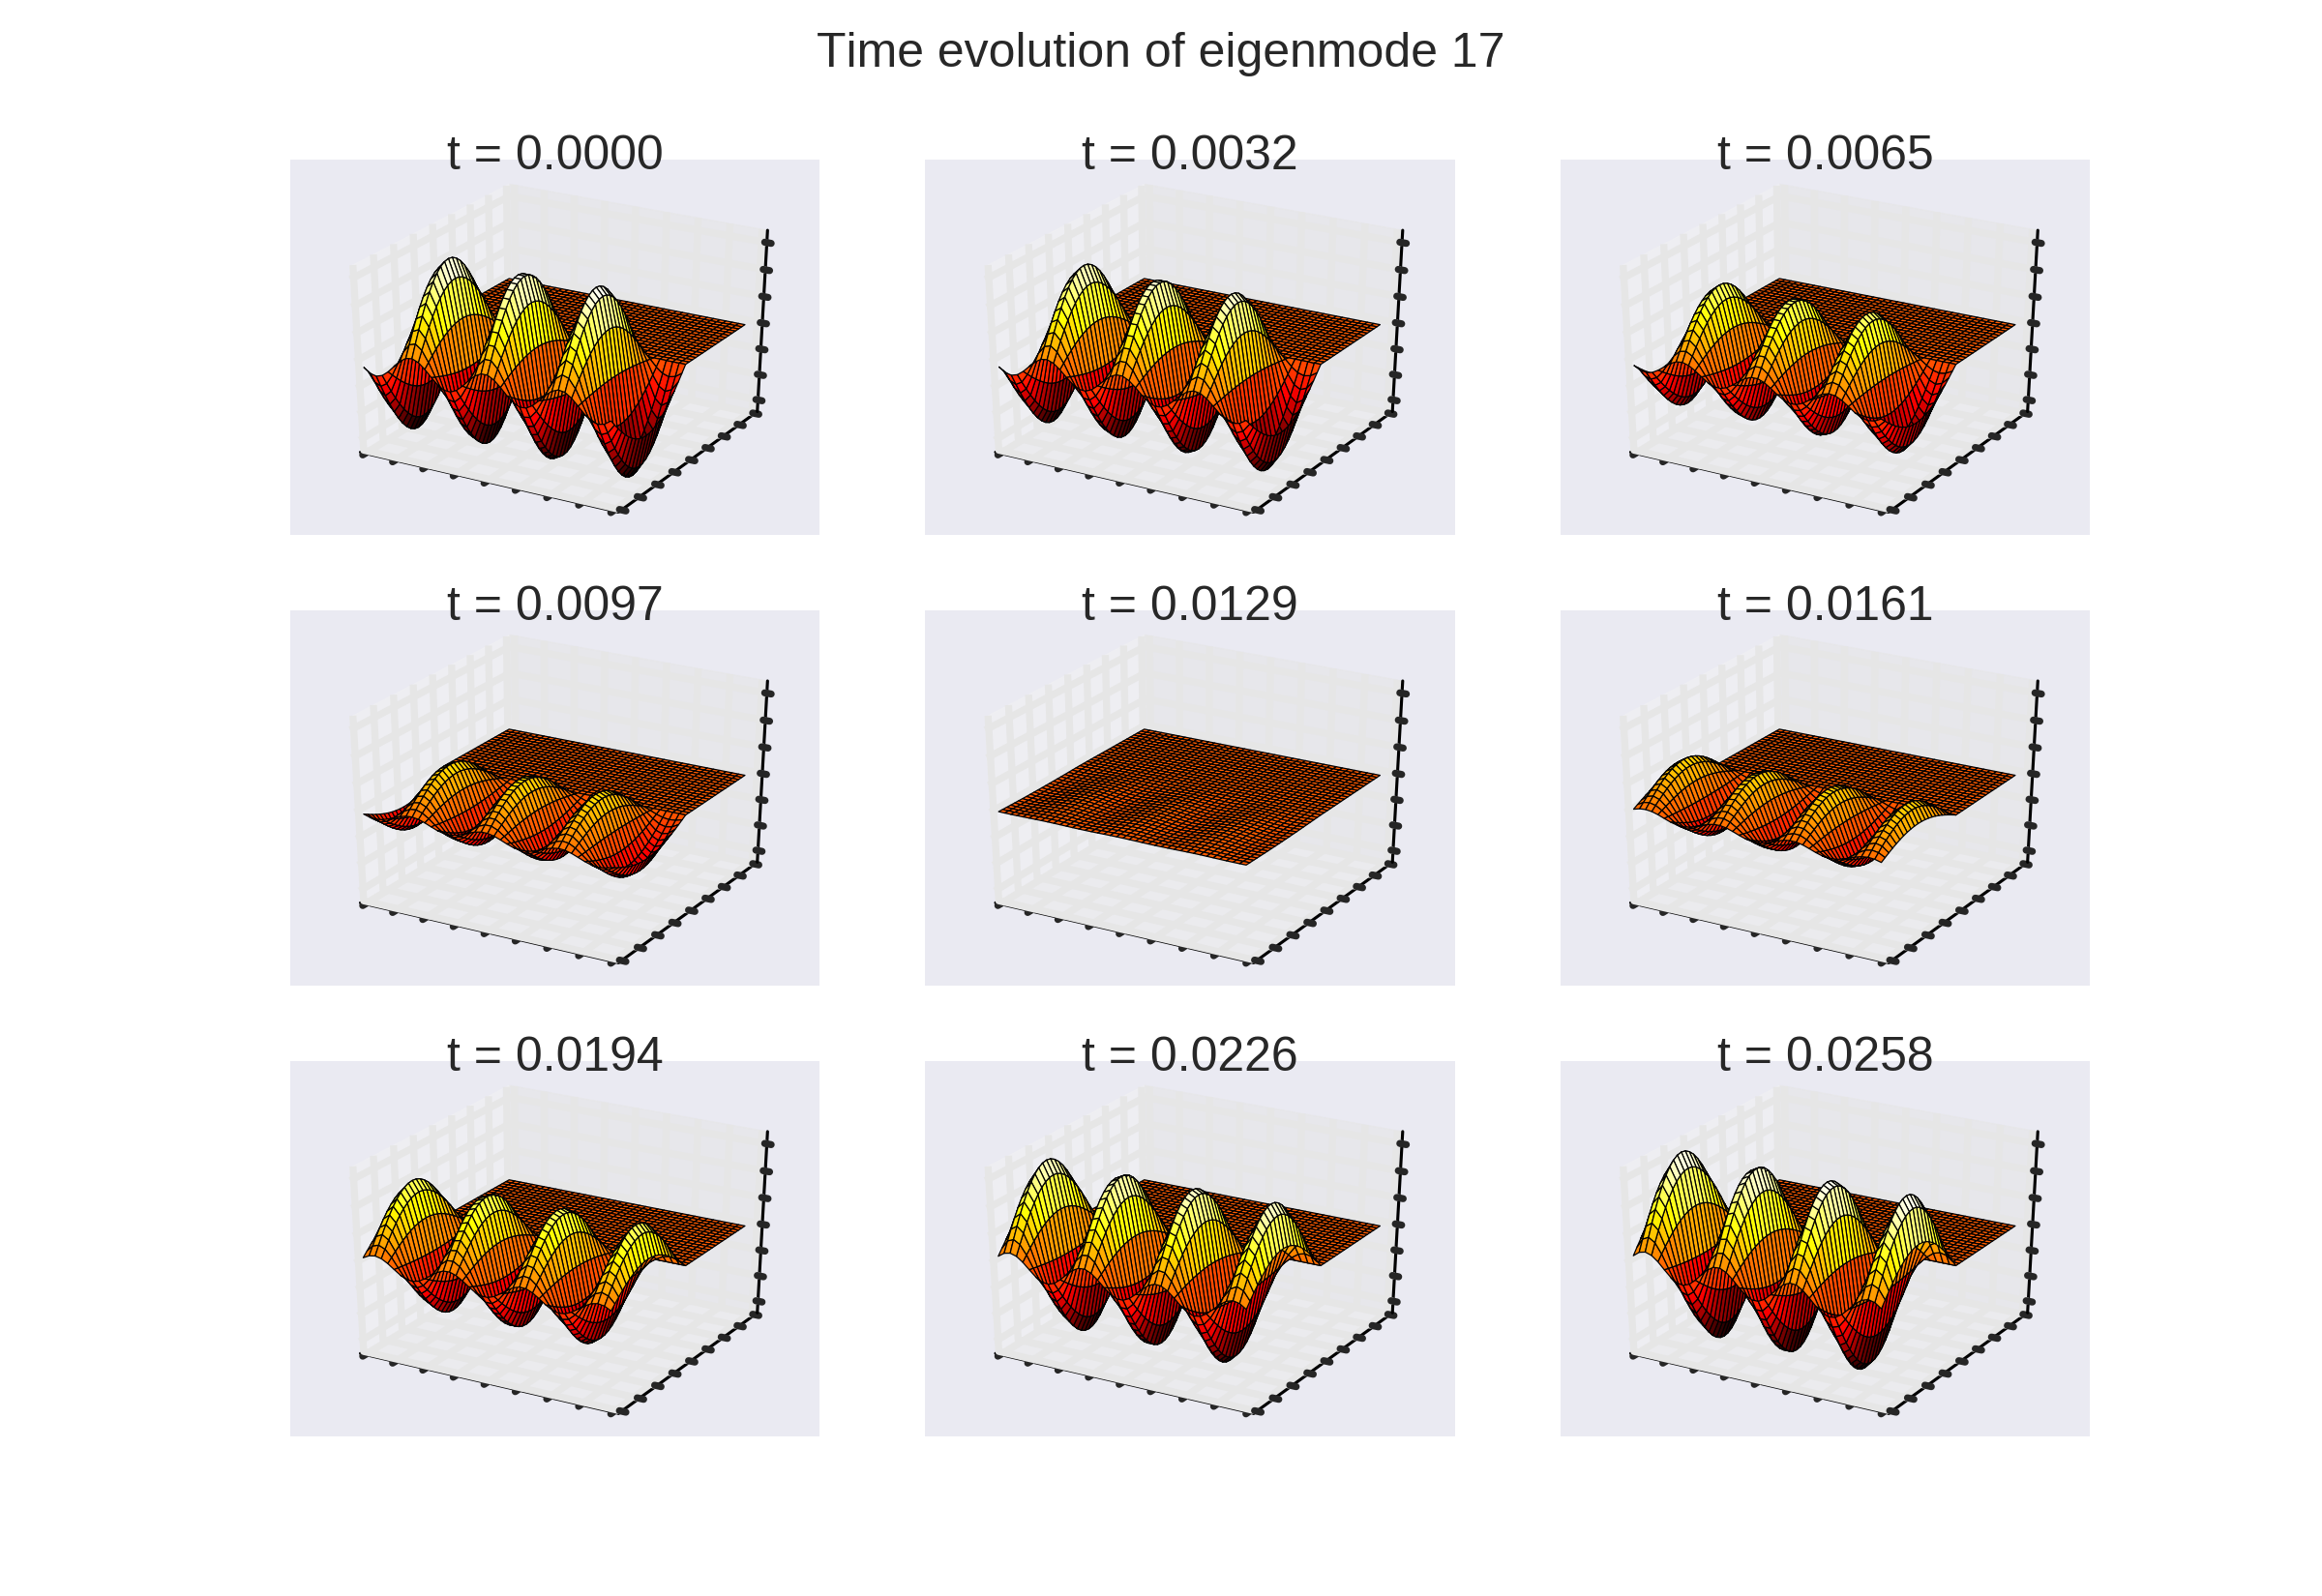
\includegraphics[width=10cm]{Pictures/time_evolution_r.png}
\caption{Some of the first time evolution calculated for a rectangular domain sorted by their frequencies.}
\label{fig:time_evolution_r}
\end{figure}

\begin{figure}
\centering
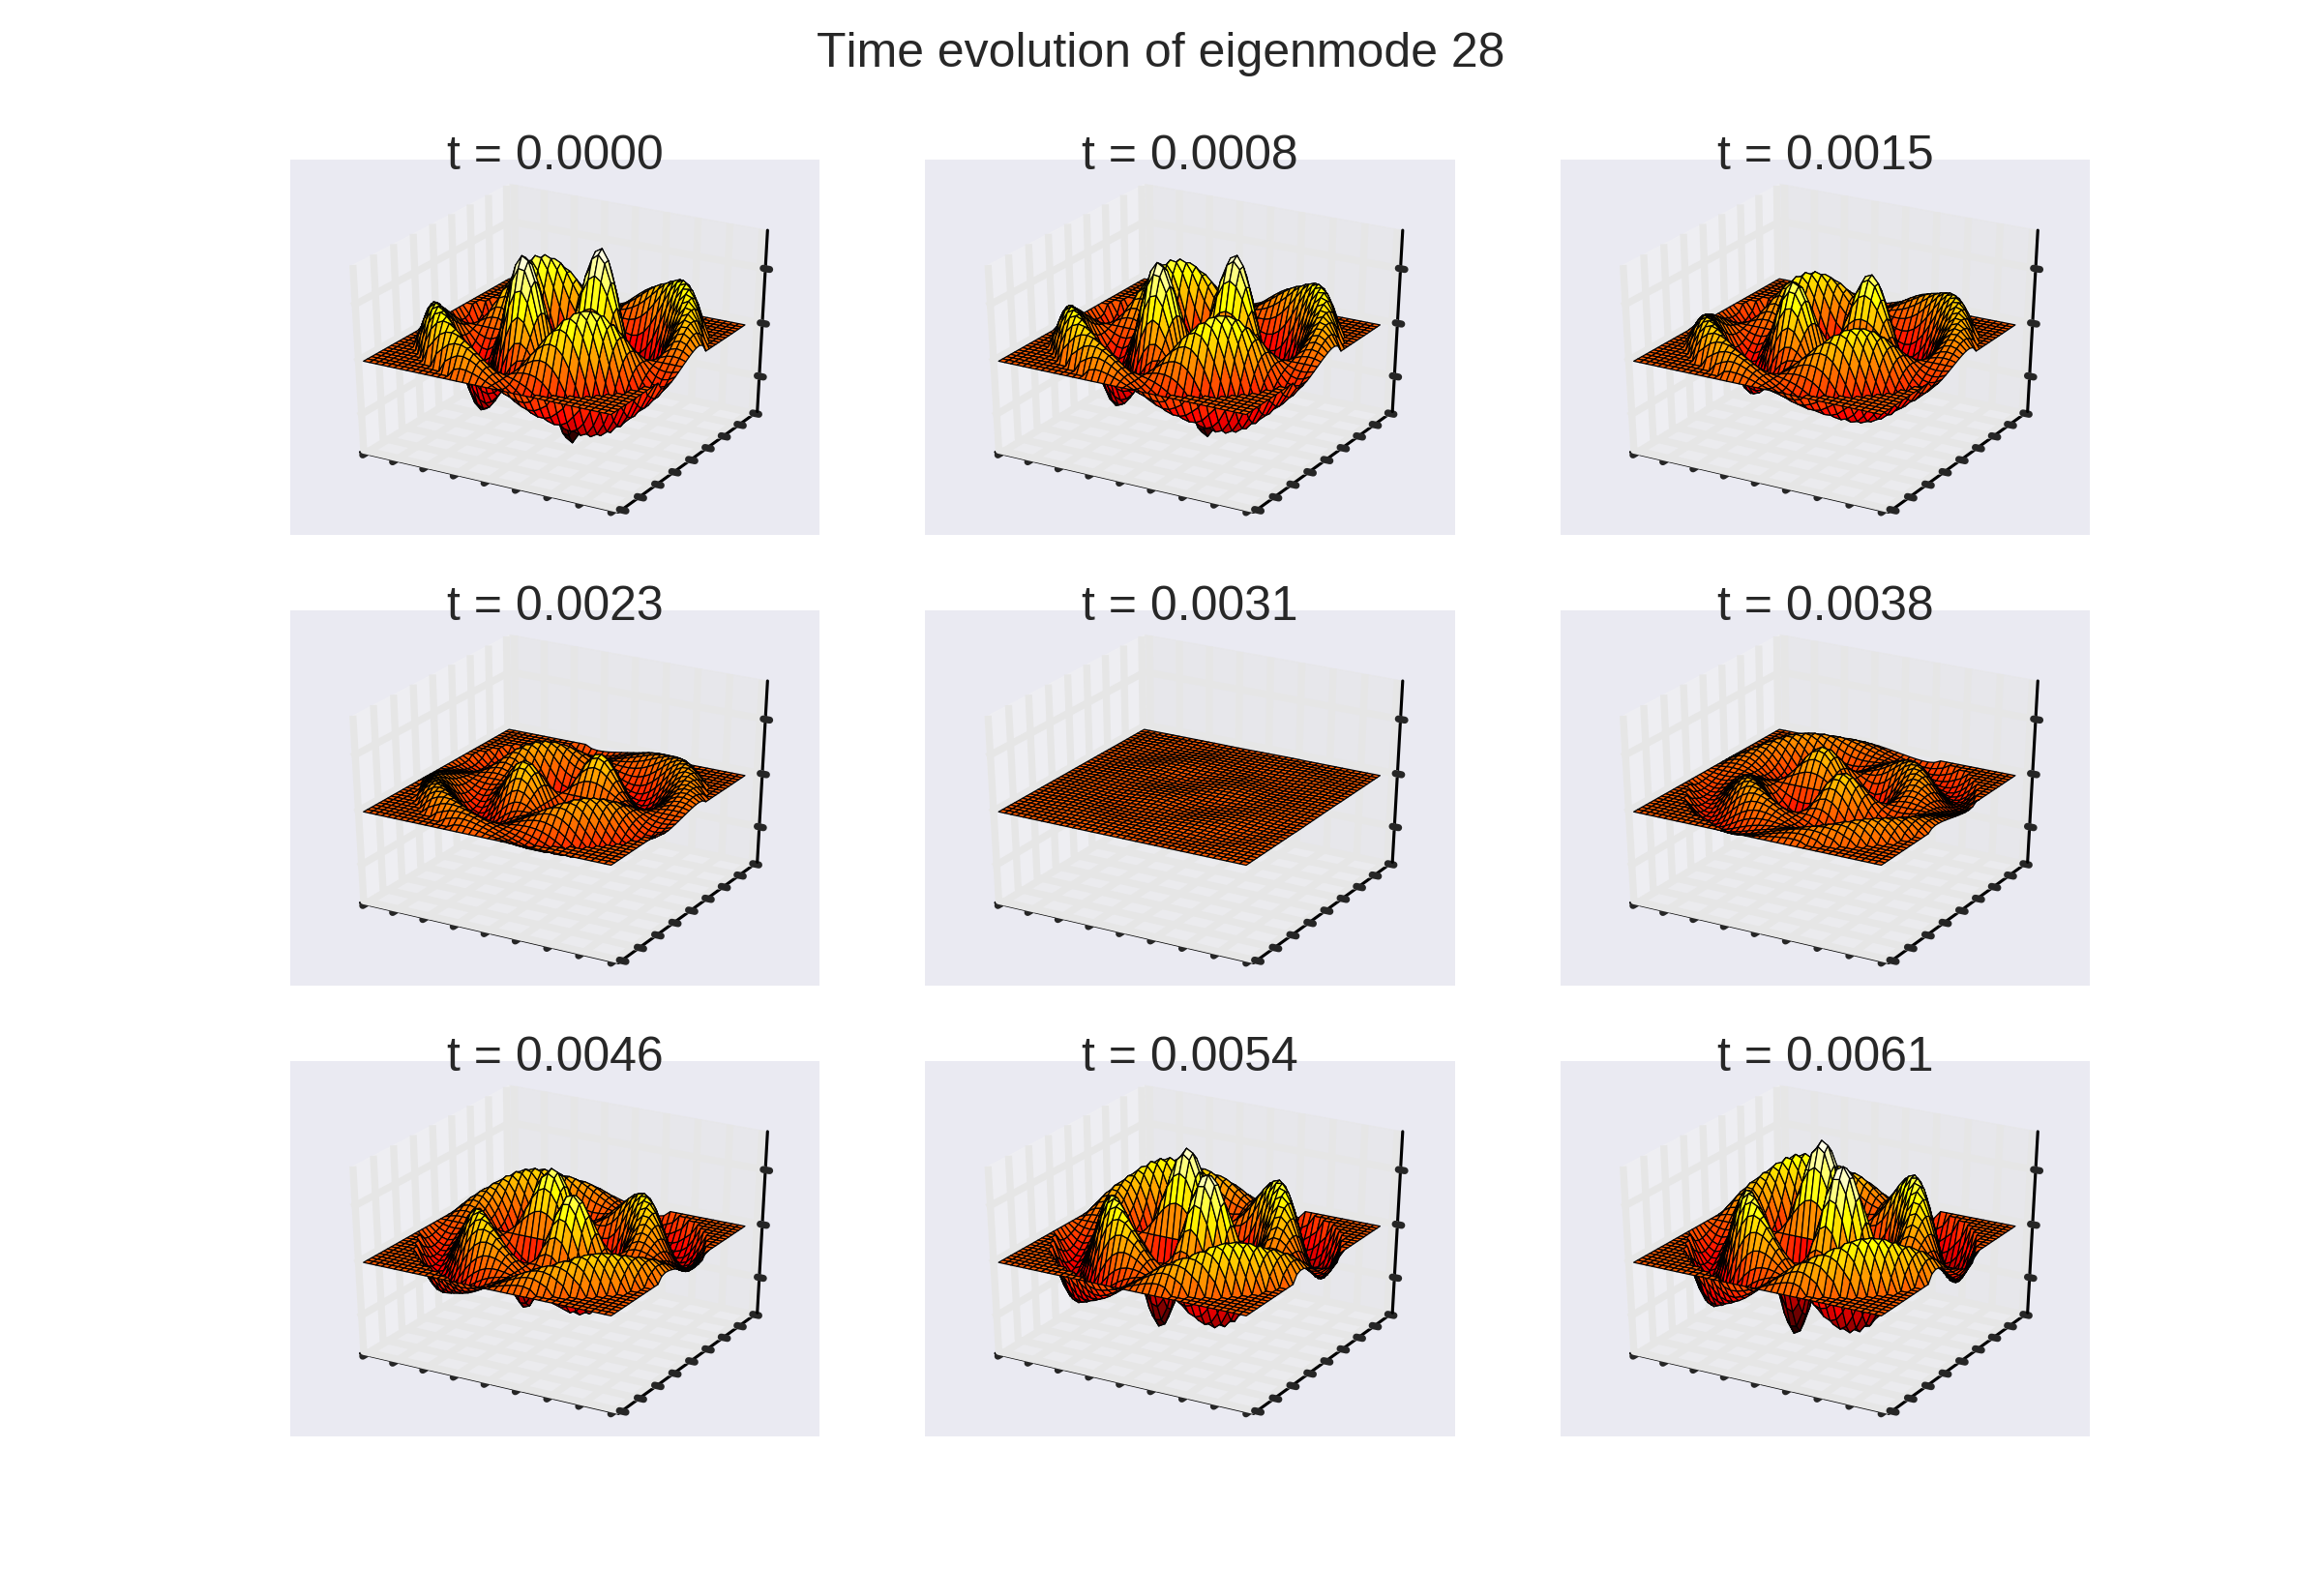
\includegraphics[width=10cm]{Pictures/time_evolution_c.png}
\caption{Some of the first time evolution calculated for a circular domain sorted by their frequencies.}
\label{fig:time_evolution_c}
\end{figure}


\section{Schr\"odinger's equation}

The time-independent Sch\"odinger equation for a single particle in a potential $V(x)$ is:

\begin{equation} \label{eq:schrodinger}
    -\frac{\hbar^2}{2m} \nabla^2 \psi(x) + V(x) \psi(x) = E \psi(x).
\end{equation}

This is an eigenvalue problem: there are infinitely many solutions $\psi_n(x)$, each with a different energy $E_n$. But the distinct $E_n$ are discrete values, the particle cannot have every energy. We will calculate the wave equations $\psi_n(x)$ and their energies $E_n$ by discretizing eq. \ref{eq:schrodinger}.

Setting $\hbar = m = 1$ and using a centered finite difference method for the second spatial derivative, we find:

\begin{equation} \label{eq:discrete_schrodinger}
    (2 + 2 \Delta x^2 V(x)) \psi_i - \psi_{i-1} - \psi_{i+1} = 2 \Delta x^2 E \psi_i.
\end{equation}

We will first look at the infinite potential well, that is defined as:

\begin{equation} \label{eq:inf_pot} 
    V(x) = 0 \text{ if} -a \leq x \leq x, \text{ infinite otherwise}
\end{equation}

We discretize space from $-a$ to $a$ with the points $i = 1, 2, \dots, N$, where $\Delta x = 2 a/ N$ and $x(i) = -a + i  \Delta x$. We assume that $\psi(0) = \psi(N) = 0$, this models infinite potential barriers at the boundaries.

We can write eq. \ref{eq:discrete_schrodinger} explicitly for all $i = 1, 2, \dots, N$ and derive a $N \times N$ matrix:

\begin{equation} \label{eq:schrodinger_eigenvalue}
\left[
\begin{array}{ccccccc}
\phi & -1 & 0 & 0 & 0 & \dots & 0\\
-1 & \phi & -1 & 0 & 0 & \dots & 0\\
0 & -1 & \phi & -1 & 0 & \dots & 0\\
\vdots & \vdots & \vdots & \vdots & \vdots & \vdots & \vdots\\
0 & \dots & 0 & 0 & -1 & \phi & -1\\
0 & \dots & 0 & 0 & 0 & -1 & \phi
\end{array}
\right]
\begin{bmatrix*}
\psi_1 \\
\psi_2 \\
\vdots \\
\psi_N \\
\end{bmatrix*}
=
2\Delta x^2 \vect{E}
\begin{bmatrix*}
\psi_1 \\
\psi_2 \\
\vdots \\
\psi_N \\
\end{bmatrix*},
\end{equation}

where $\phi = 2 + 2 \Delta x ^2 V(x)$. Note that in the first and last row we've used that $\psi_0 = \psi_N = 0$. In this form, the problem can be readily solved using standard routines to find the eigenvalues and eigenvectors.

We've solved this for $N = 200$ and the infinite potential well as defined in eq. \ref{eq:inf_pot}, the computed probability distribution functions (the eigenvectors) can be seen in figure \ref{fig:infinite} in green. In blue are the real, analytic solutions. We see that they are very close. The potential is invisible because it is everywhere zero. The analytic solutions were computed using\footnote{adapted from equation 2.28 in \cite{griffiths}}:

\begin{equation} \label{eq:inf_pot_analytic}
    \psi_n(x) = \sqrt{\frac{2}{a}} \sin(n \pi (x - a) / (2 a)),
\end{equation}
where $n$ is the quantum number. Increasing numbers of $n$ belong to increasing energies $E_n$. For the infinite potential well we also have an analytic expression for the allowed energies\footnote{from equation 2.27 in \cite{griffiths}}:

\begin{equation} \label{eq:inf_pot_en}
    E_n = \frac{n^2 \pi^2 \hbar^2}{2m(2a)^2}.
\end{equation}

\begin{figure}
\centering
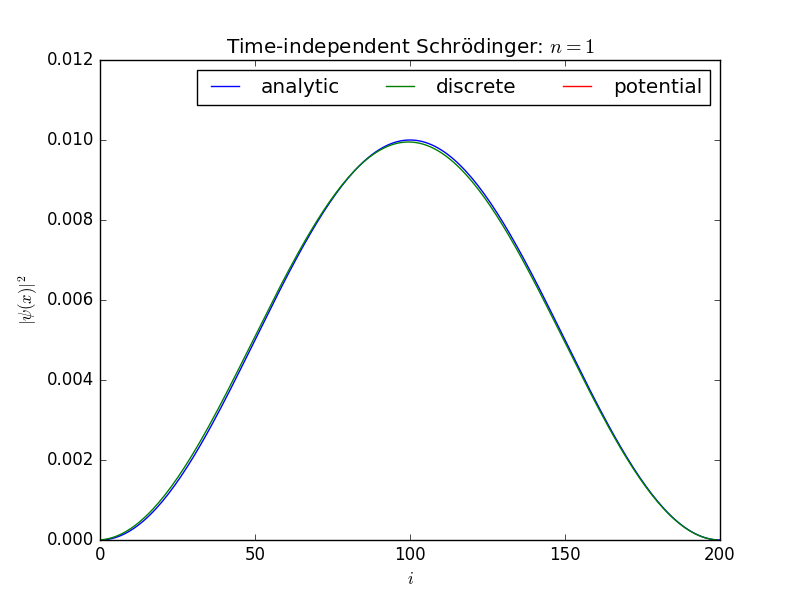
\includegraphics[width=6cm]{infinite_1}
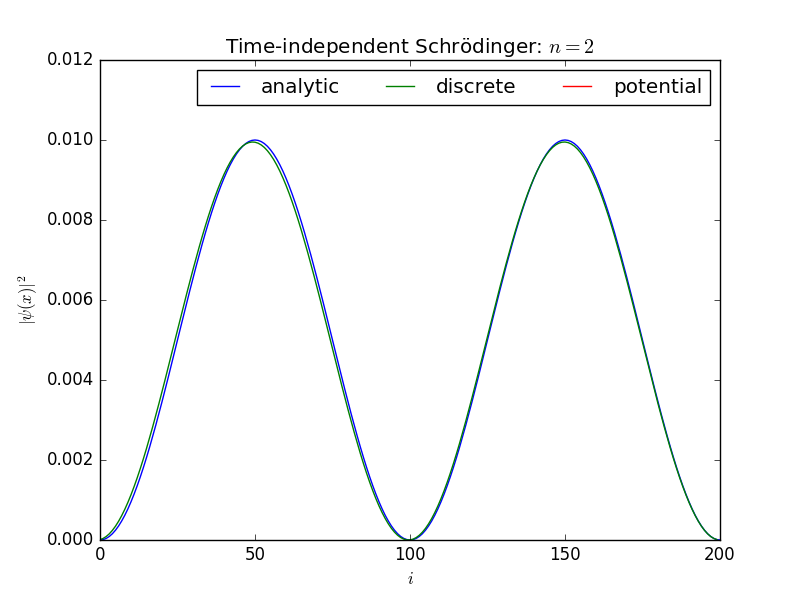
\includegraphics[width=6cm]{infinite_2}
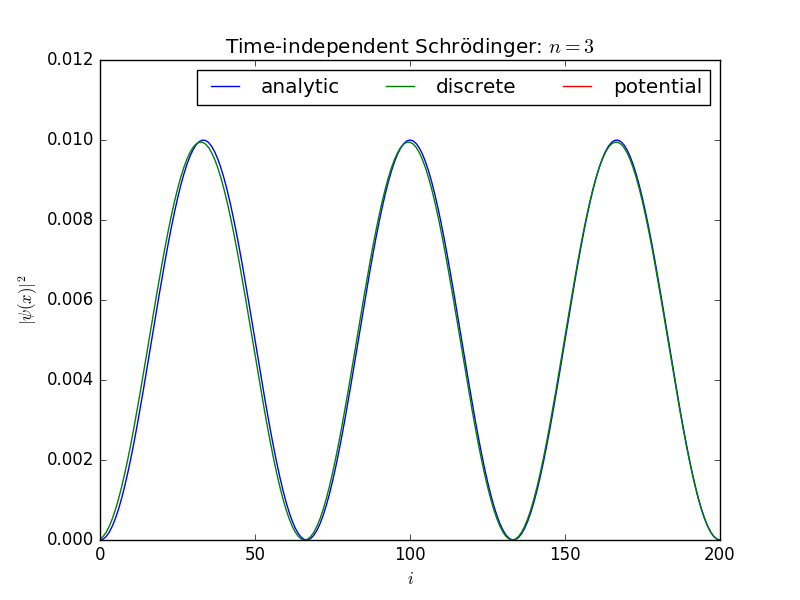
\includegraphics[width=6cm]{infinite_3}
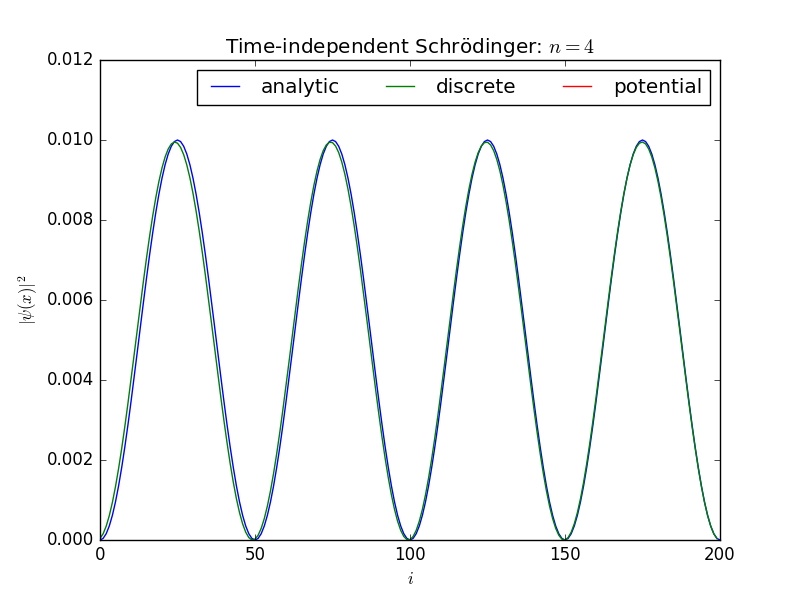
\includegraphics[width=6cm]{infinite_4}
\caption{The solutions to the time-independent Schr\"odinger equation computed analytically and by solving the eigenvalue problem from eq. \ref{eq:schrodinger_eigenvalue}.}
\label{fig:infinite}
\end{figure}

In figure \ref{fig:energies} we see the corresponding eigenvalues of the solutions in figure \ref{fig:infinite} with the analytic values calculated using eq. \ref{eq:inf_pot_en}. We see that for low eigenvalues till 50 the calculated and real values mostly overlap. From then on they start to diverge and the calculated energies reach a plateau. It seems that here only the first $N/4$ calculated energy values can be trusted.

\begin{figure}
\centering
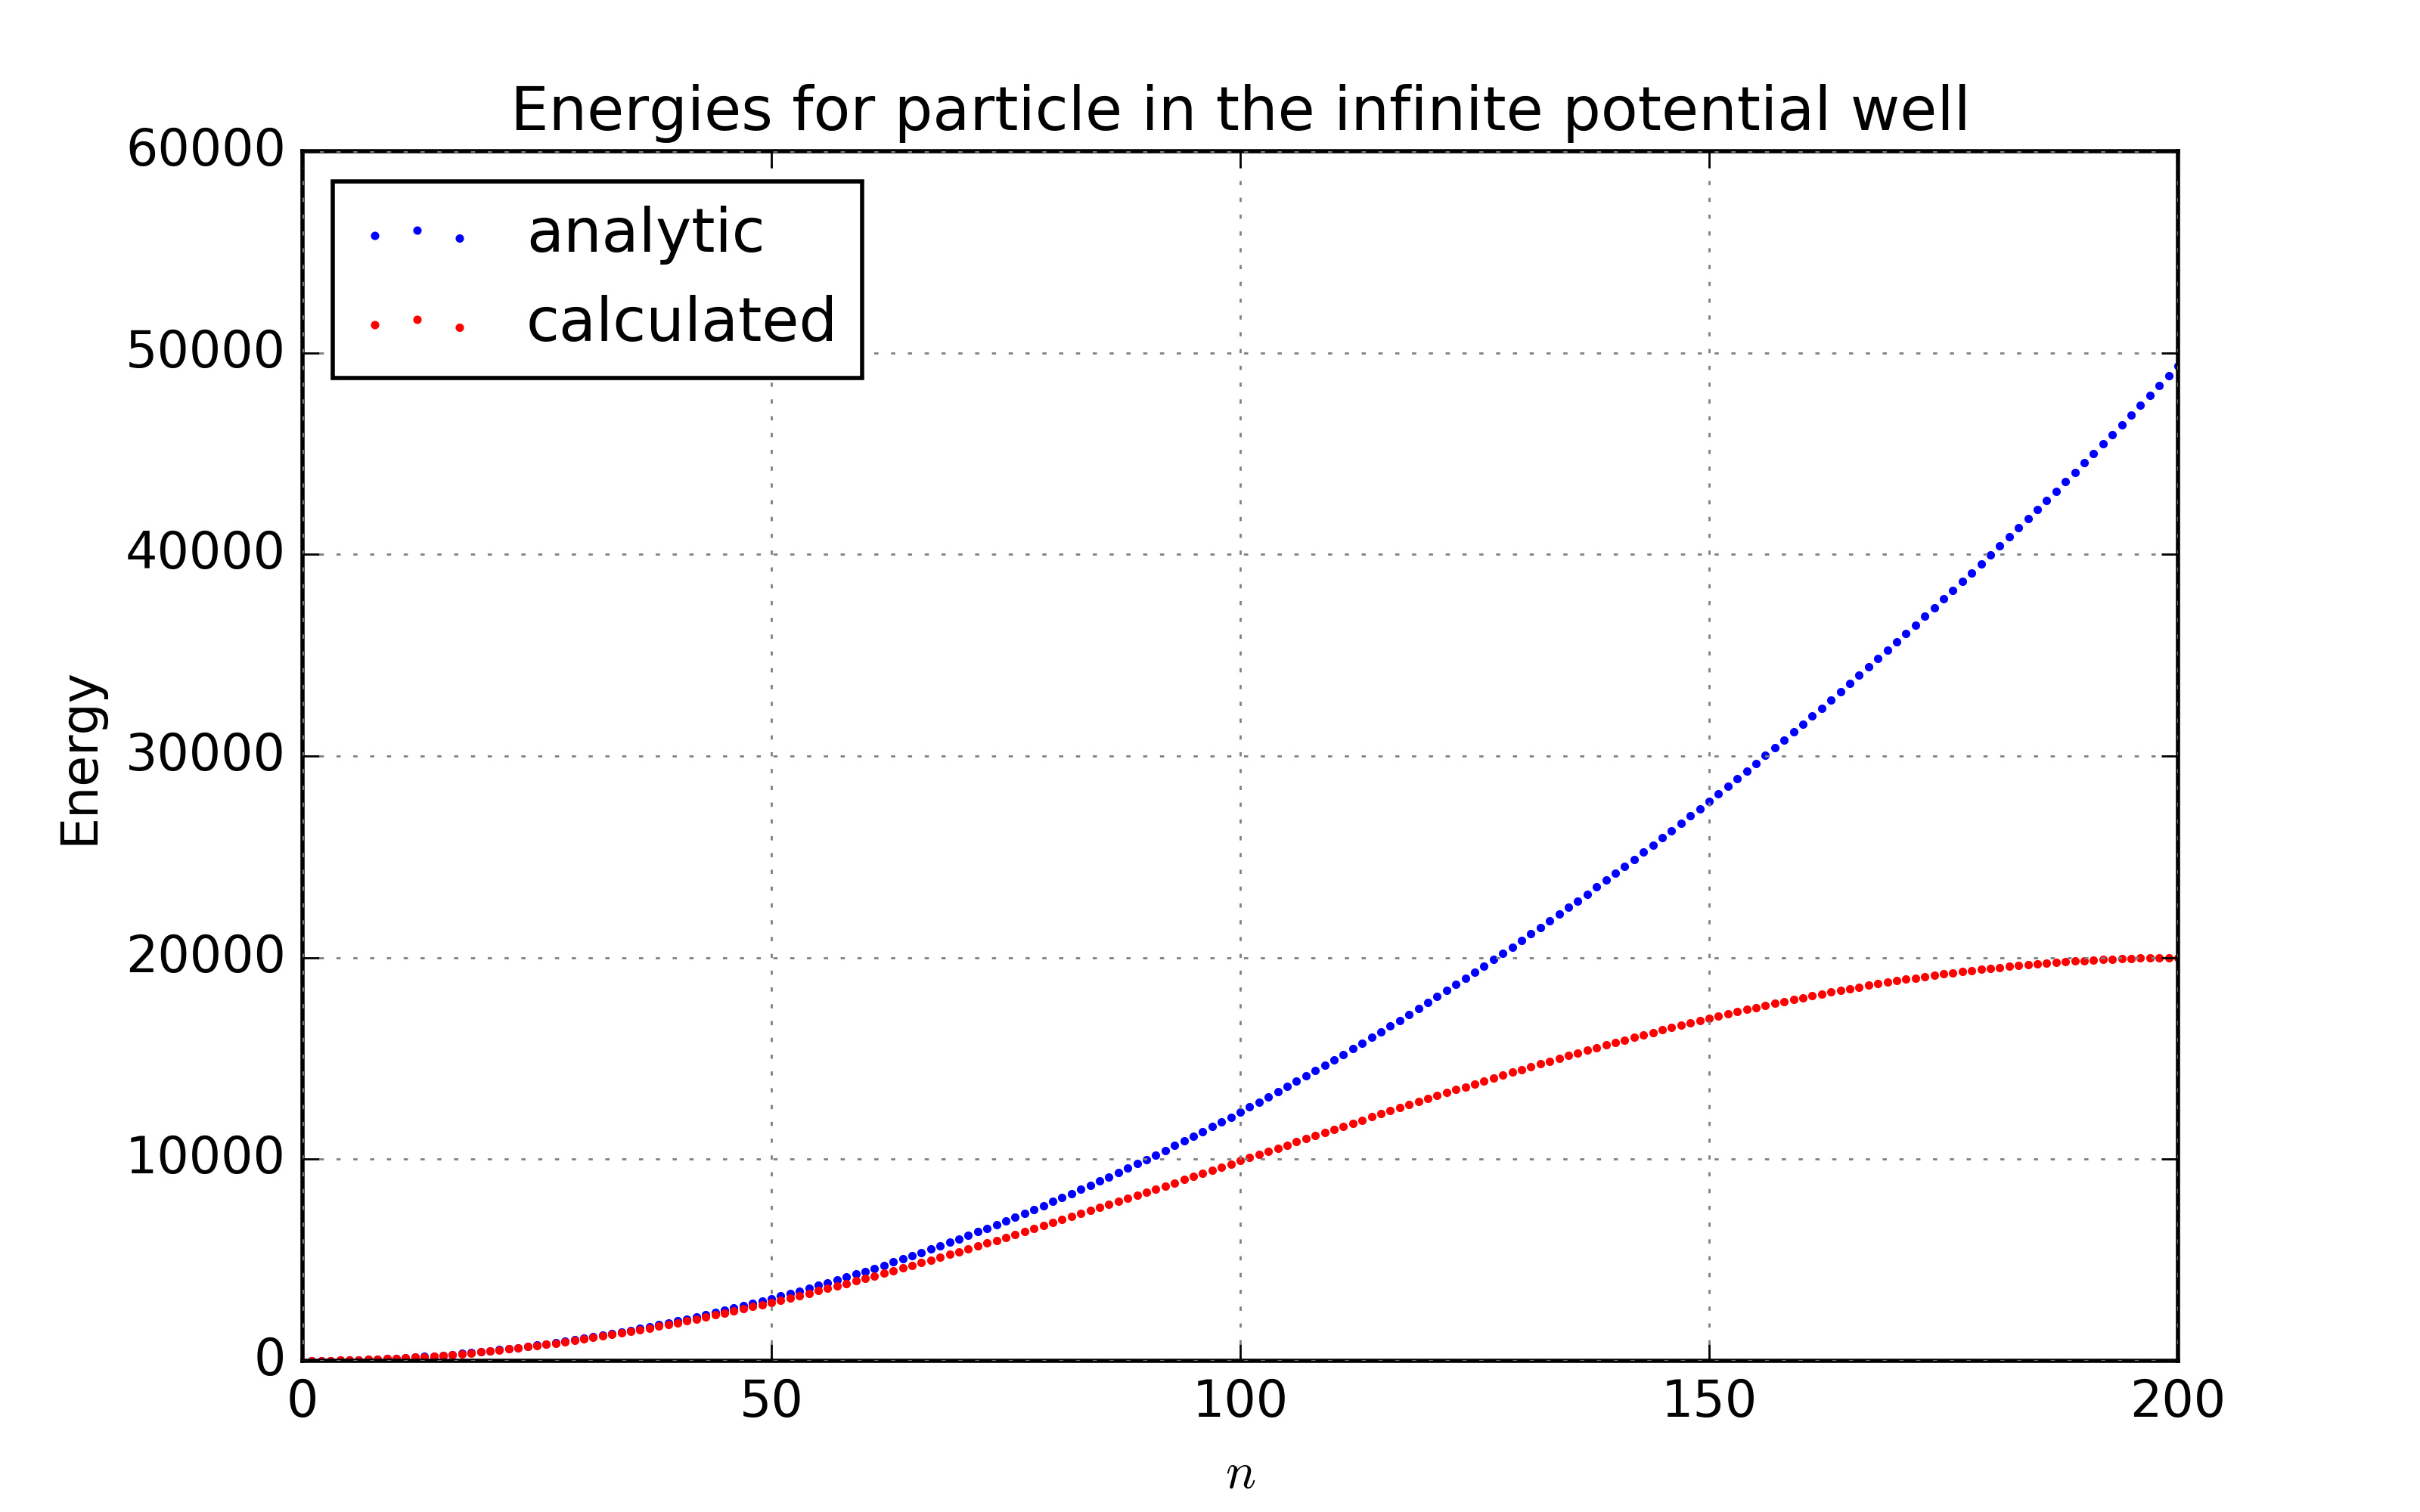
\includegraphics[width=10cm]{energies}
\caption{The calculated and analytic energies for a particle in an infinite potential well.}
\label{fig:energies}
\end{figure}

Let's now look at a finite potential well that is defined as:

\begin{equation}
    V(x) = 0 \text{ if} -a \leq x \leq a, \text{ $V_0$ otherwise},
\end{equation}
with $V_0 = 10$. The only difference in the implementation are the values for $\phi$ in the first and last rows of \ref{eq:schrodinger_eigenvalue}. The energies are a bit higher than for the infinite potential well and the wave equations are very similar to those in figure 
\ref{fig:infinite}. Because these results are rather uninteresting, we will magnify the effect of the finite potential by adjusting its domain:

\begin{equation} \label{eq:finite_pot}
    V(x) = 0 \text{ if} -4a/5 \leq x \leq 4a/5, \text{ $V_0$ otherwise},
\end{equation}
again with $V_0=10$. Now more rows in matrix \ref{eq:schrodinger_eigenvalue} model the effect of the finite potential well. The resulting wave functions can be seen in figure \ref{fig:finite}. We observe tunneling: there is a non-zero probability of the particle crossing the potential barrier.

\begin{figure}
\centering
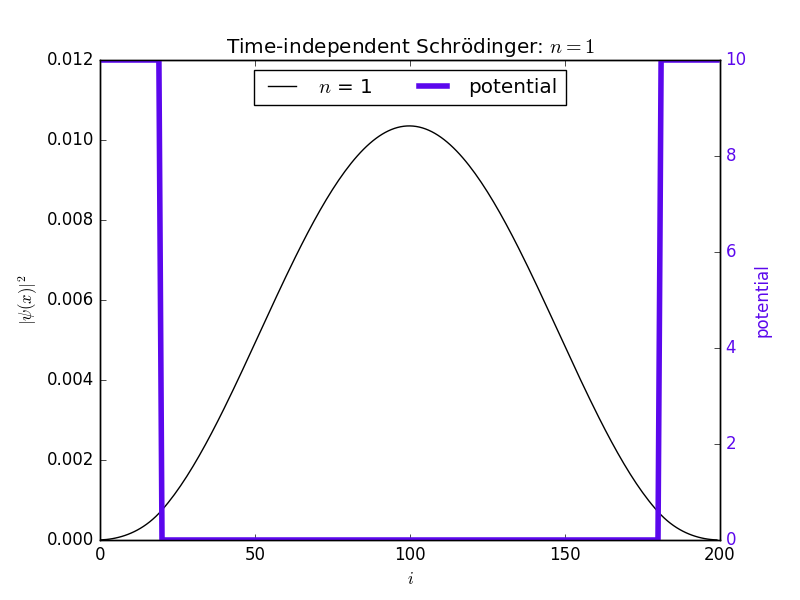
\includegraphics[width=6cm]{finite_scaled_1}
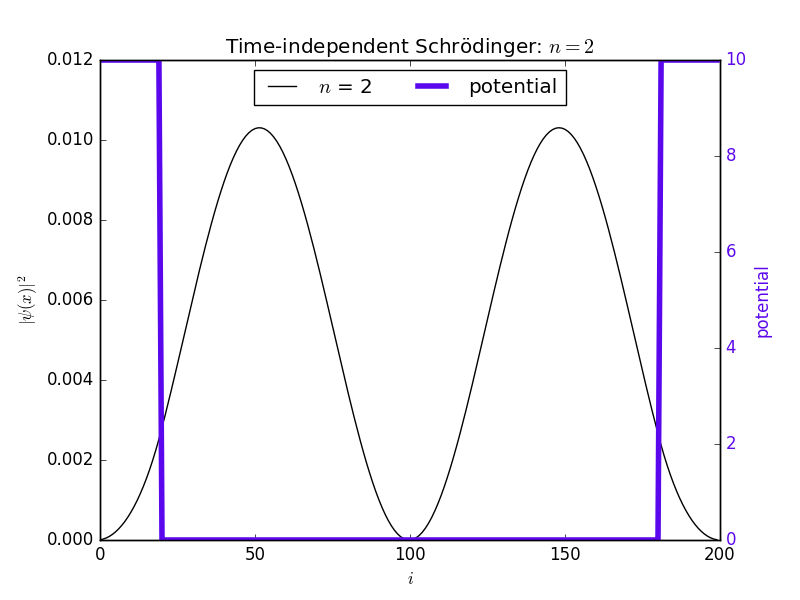
\includegraphics[width=6cm]{finite_scaled_2}
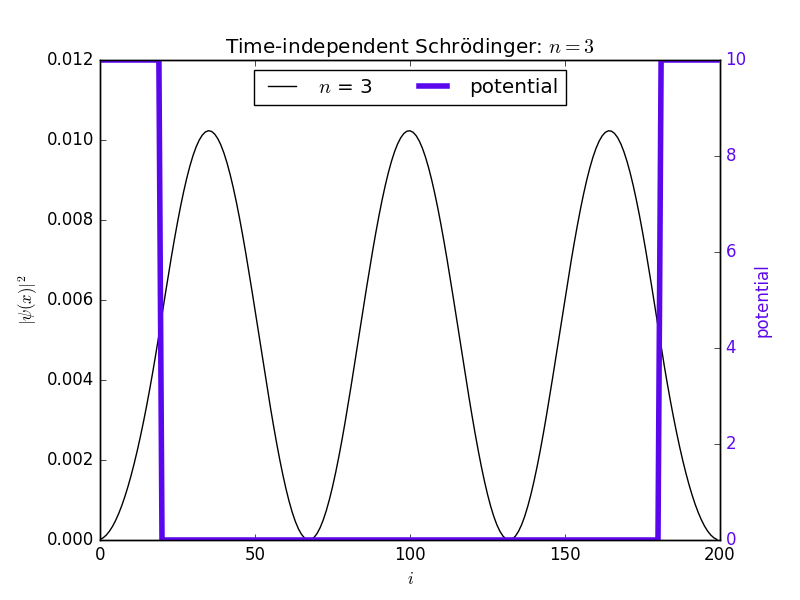
\includegraphics[width=6cm]{finite_scaled_3}
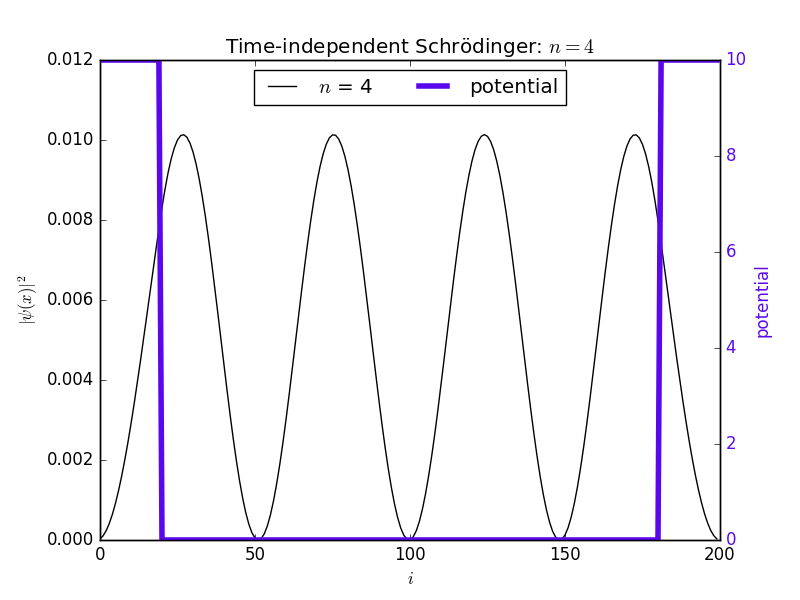
\includegraphics[width=6cm]{finite_scaled_4}
\caption{The solutions to the time-independent Schr\"odinger equation found by solving the eigenvalue problem from eq. \ref{eq:schrodinger_eigenvalue} with the finite potential well defined in eq. \ref{eq:finite_pot}. The potential is displayed in purple.}
\label{fig:finite}
\end{figure}

Lastly we look at a parabolic potential well defined as:
\begin{equation} \label{eq:finite_pot}
    V(x) = bx^2,
\end{equation}
where $b$ specifies the magnitude of the potential. In figure \ref{fig:parabolic} we see the wave equations for a particle in such potential with $b=500$. When comparing with the wave equations in figure \ref{fig:infinite}, we see that the parabolic potential pushes the particle to the middle, where the potential and thus the energy of the particle would be lowest.

The energies for both the finite and parabolic potentials are a bit higher than for the infinite potential. We don't explicitly show them because they would almost coincide with the infinite potential will as calculated in \ref{fig:energies}.

\begin{figure}
\centering
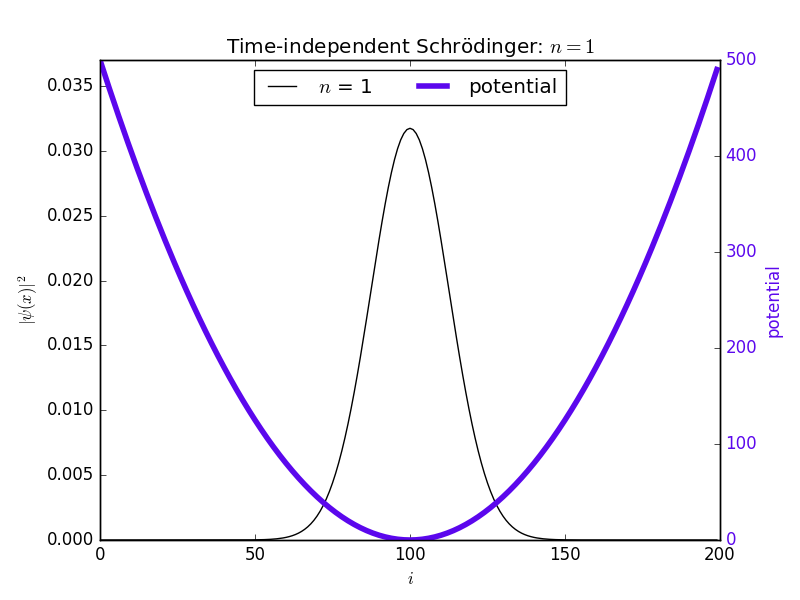
\includegraphics[width=6cm]{parabolic_1}
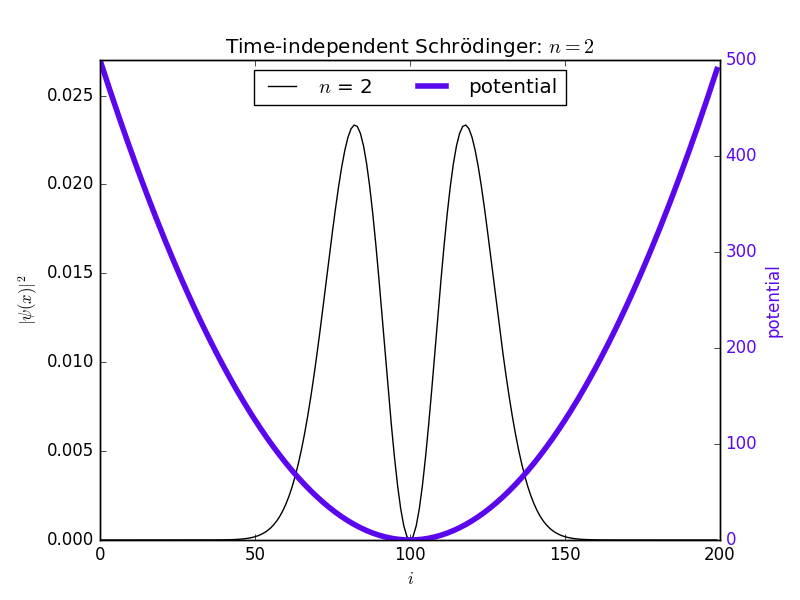
\includegraphics[width=6cm]{parabolic_2}
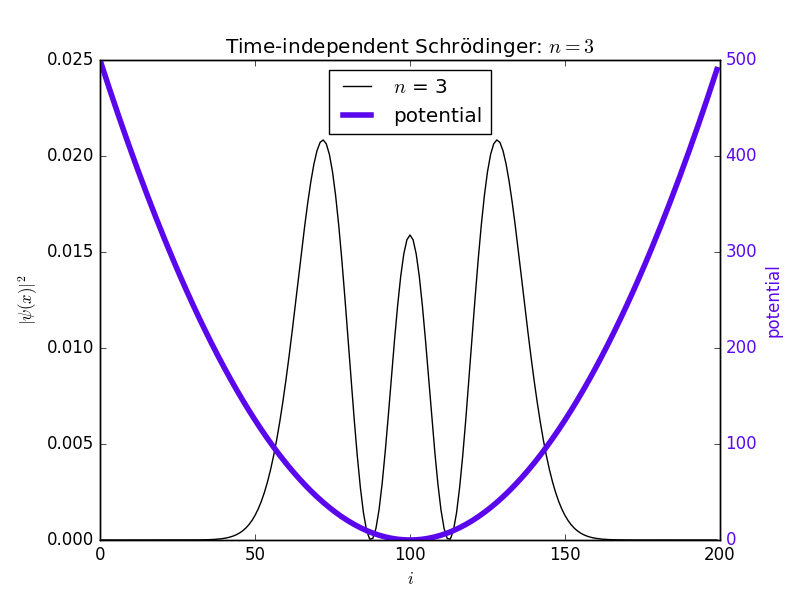
\includegraphics[width=6cm]{parabolic_3}
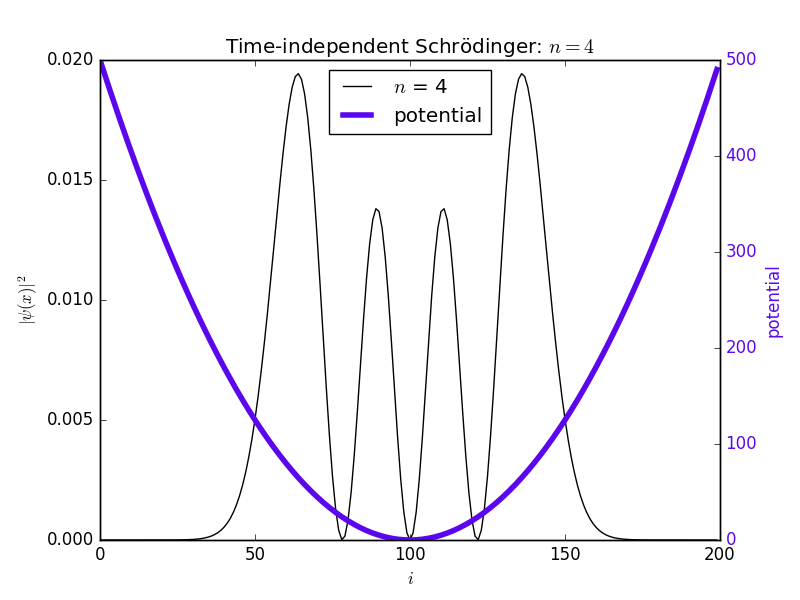
\includegraphics[width=6cm]{parabolic_4}
\caption{Solutions to the time-independent Schr\"odinger equation for a particle in a parabolic potential well.}
\label{fig:parabolic}
\end{figure}

\section{Direct methods for solving steady state problems}

Here we look at solving the diffusion equation for the steady state using a direct method. The diffusion equation is:
\begin{equation*} \label{eq:diffusion}
    \frac{\partial c}{\partial t} = \left( \frac{\partial^2}{\partial x^2} + \frac{\partial^2}{\partial y^2} \right) c,
\end{equation*}
for steady states we have $\partial c/ \partial t = 0$, so we have to solve $\nabla^2 c = 0$. We construct a matrix $M$ for the $\nabla^2$ as described in the appendix. We take a domain of 4 by 4, and discretize the $x$ and $y$ directions with $N=80$ equal units. The $M$ matrix then is a $N^2$ by $N^2$ matrix. For the boundary we construct a vector $b$ that has $N^2$ elements, where all values are zero, except the point (0.6, 1.2) which is 1. The solution for this system is shown in figure \ref{fig:diffusion}. We tried applying the circular domain by setting those pixels in $M$ that are beyond a radius of 2 to zero, but that failed because $M$ would then be a singular matrix with no solution.

\begin{figure}
\centering
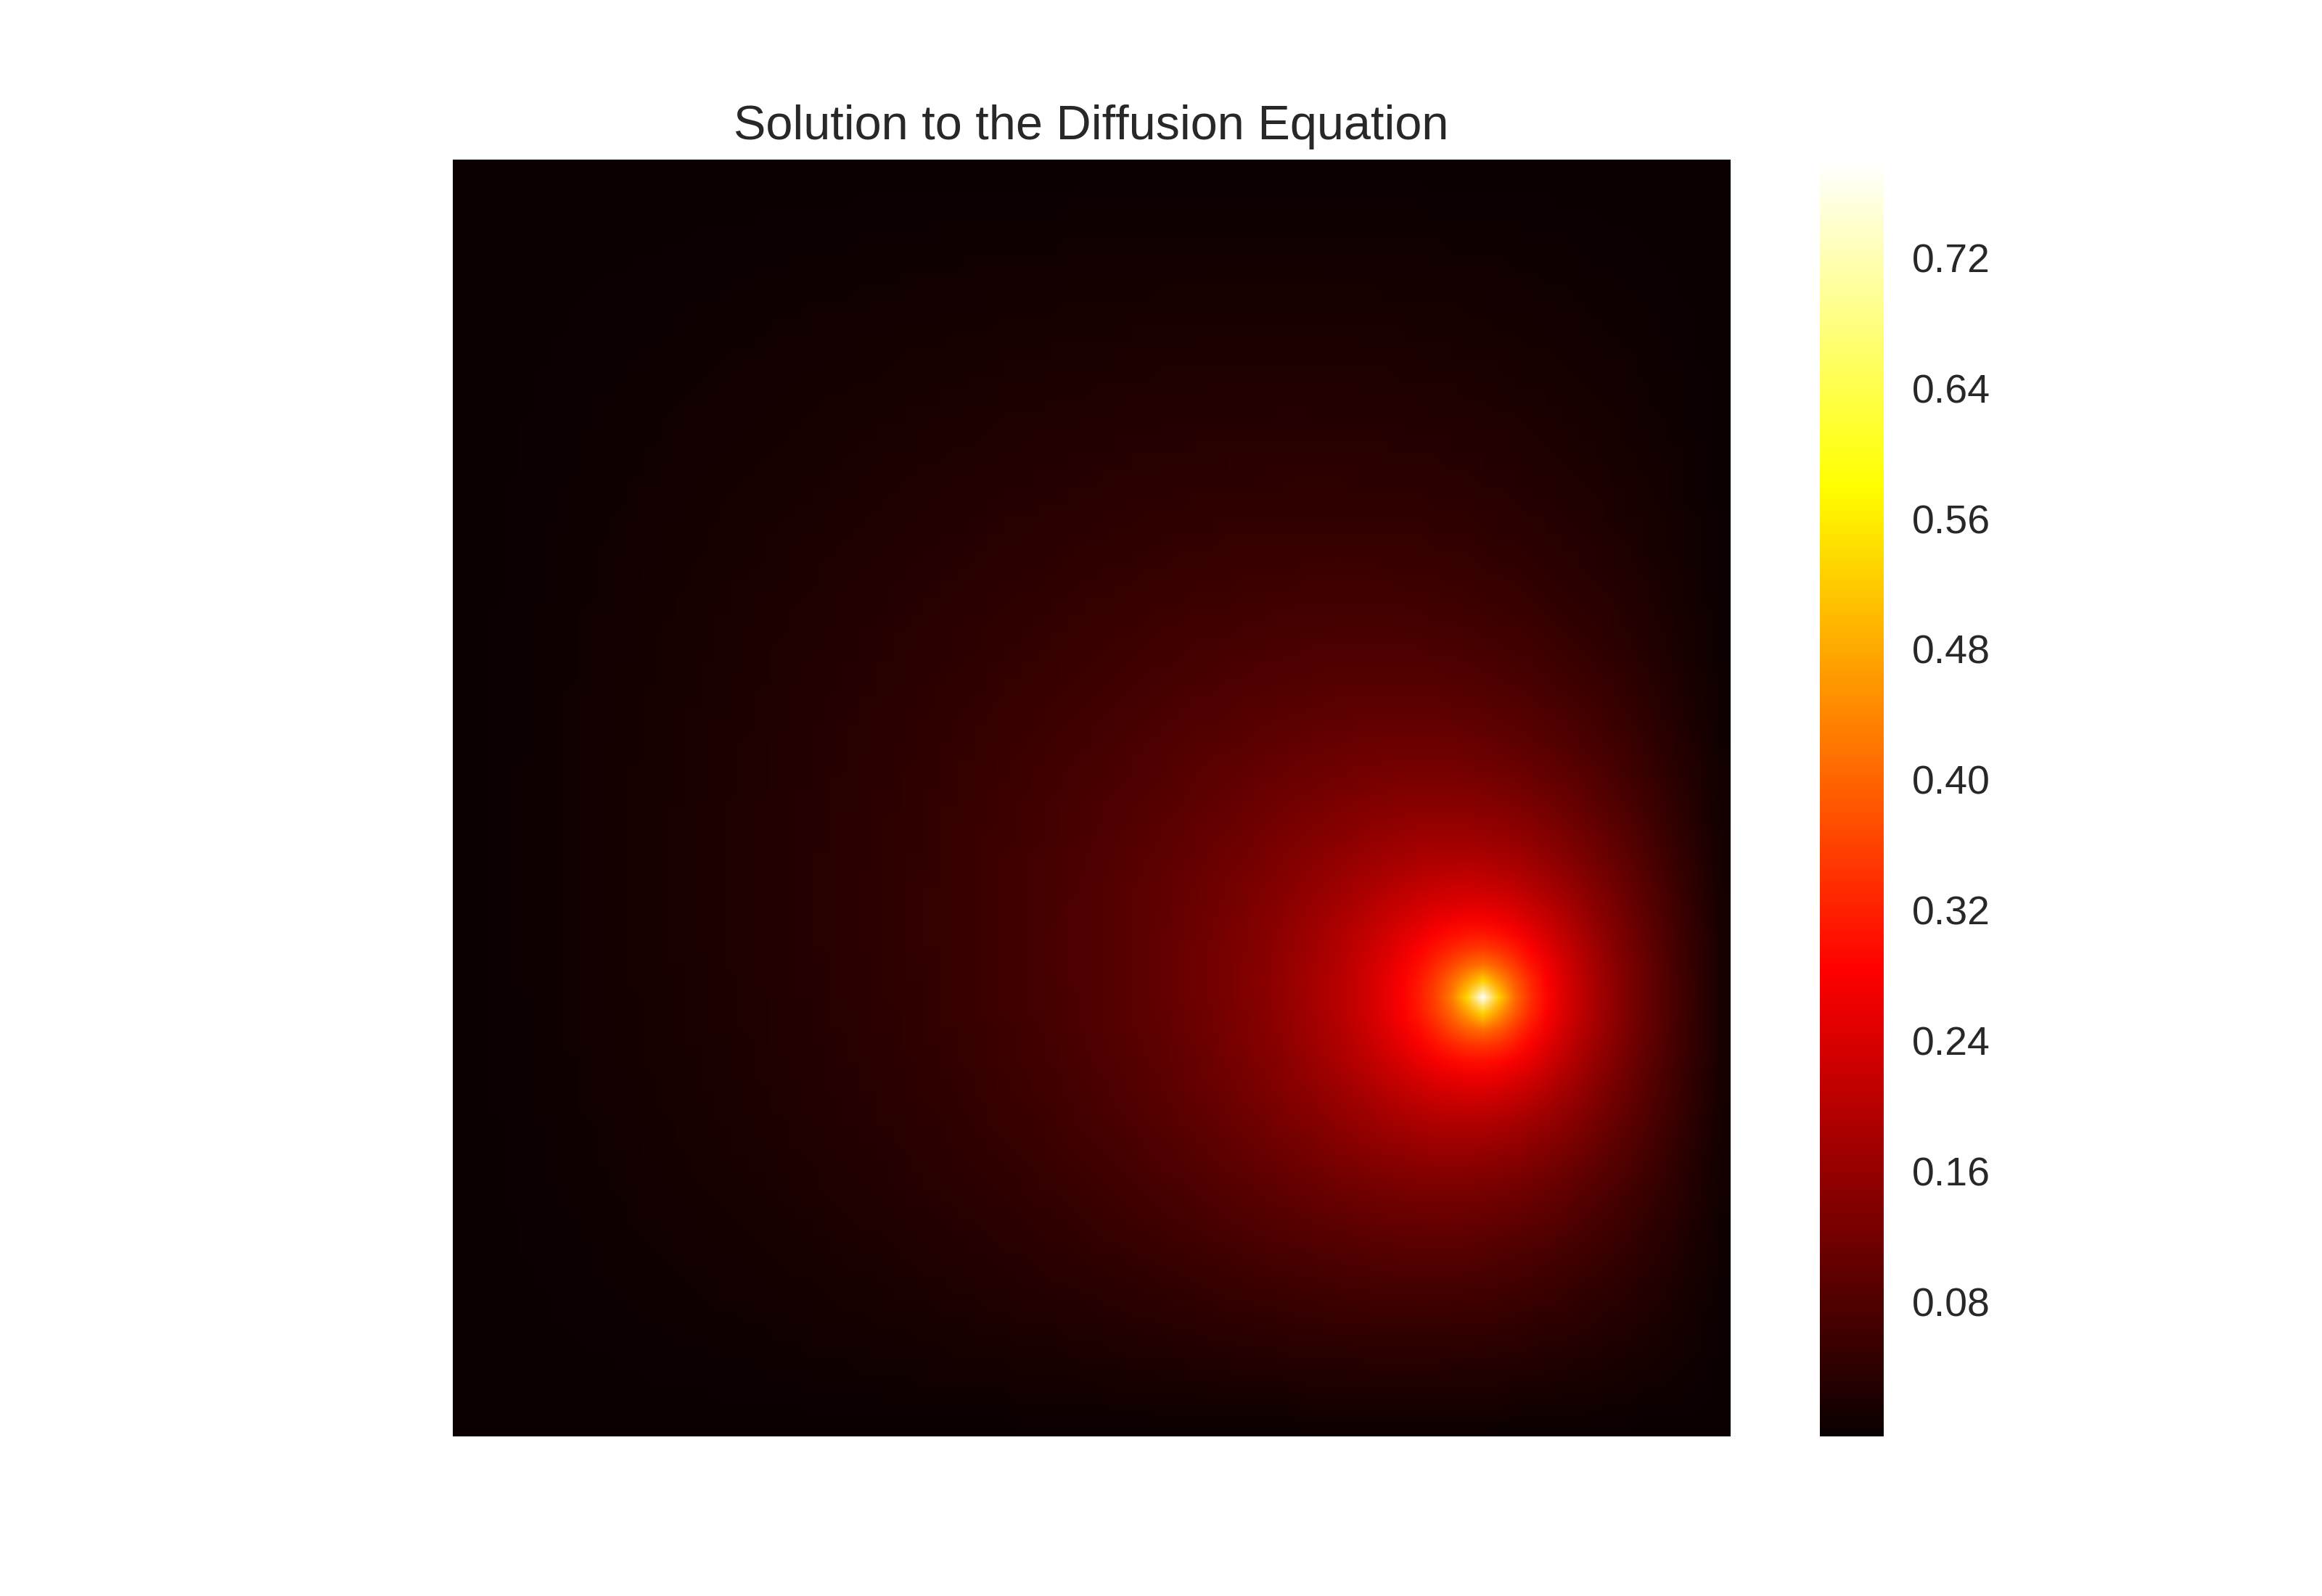
\includegraphics[width=14cm]{diffusion}
\caption{The solution to the diffusion equation. The domain for both $x$ and $y$ directions are from -2 to 2.}
\label{fig:diffusion}
\end{figure}

\newpage
\appendix
\section{Matrix representation of the wave equation}
\label{app:A}

The discretization of the two dimensional wave equation can be written in matrix form. The general form for any square systemsize is given as follows:
\begin{equation}
\left[
\begin{array}{c:c:c:c:c}
    A       &I    & 0     & \dots & 0 \\
    \hdashline
    I      &A     &I     & \ddots     & \vdots \\
    \hdashline
    0       &I     &\ddots & I & 0\\
    \hdashline
    \vdots  &\ddots &I & A    & I \\
    \hdashline
    0       &\dots  &0      & I    & A \\
\end{array}
\right ]
\begin{bmatrix*}
    v_{1,1}\\
    v_{2,1}\\
    v_{1,2}\\
    \vdots\\
    v_{N,N}
\end{bmatrix*}
=
\lambda
\begin{bmatrix*}
    v_{1,1}\\
    v_{2,1}\\
    v_{1,2}\\
    \vdots\\
    v_{N,N}
\end{bmatrix*}
\label{eq:genMatExp}
\end{equation}

Where I is the identity matrix of size $N \times N$, 0 is the zero matrix of the same size and A is an $N \times N$ matrix of the following form:

\begin{equation}
A = 
\left[
\begin{array}{rrrrr}
    -4       &1     & 0     & \dots & 0 \\
    1      &-4      &1     & \ddots     & \vdots \\
    0       &1     &\ddots &\ddots& 0\\
    \vdots  &\ddots &\ddots & -4    & 1 \\
    0       &\dots  &0      & 1    & -4 \\
\end{array}
\right]
\label{eq:matA}
\end{equation}

For example the full finite difference matrix in a $4 \times 4$ domain looks like this:

\begin{equation}
\left[
\tiny
\begin{array}{rrrr|rrrr|rrrr|rrrr}
    -4 & 1 & 0 & 0 & 1 & 0 & 0 & 0 & 0 & 0 & 0 & 0 & 0 & 0 & 0 & 0 \\
    1 & -4 & 1 & 0 & 0 & 1 & 0 & 0 & 0 & 0 & 0 & 0 & 0 & 0 & 0 & 0 \\
    0 & 1 & -4 & 1 & 0 & 0 & 1 & 0 & 0 & 0 & 0 & 0 & 0 & 0 & 0 & 0 \\
    0 & 0 & 1 & -4 & 0 & 0 & 0 & 1 & 0 & 0 & 0 & 0 & 0 & 0 & 0 & 0 \\
\hline
    1 & 0 & 0 & 0 & -4 & 1 & 0 & 0 & 1 & 0 & 0 & 0 & 0 & 0 & 0 & 0 \\
    0 & 1 & 0 & 0 & 1 & -4 & 1 & 0 & 0 & 1 & 0 & 0 & 0 & 0 & 0 & 0 \\
    0 & 0 & 1 & 0 & 0 & 1 & -4 & 1 & 0 & 0 & 1 & 0 & 0 & 0 & 0 & 0 \\
    0 & 0 & 0 & 1 & 0 & 0 & 1 & -4 & 0 & 0 & 0 & 1 & 0 & 0 & 0 & 0 \\
    \hline
     0 & 0 & 0 & 0 &1 & 0 & 0 & 0 & -4 & 1 & 0 & 0 & 1 & 0 & 0 & 0 \\
     0 & 0 & 0 & 0 & 0 & 1 & 0 & 0 & 1 & -4 & 1 & 0 & 0 & 1 & 0 & 0 \\
     0 & 0 & 0 & 0 & 0 & 0 & 1 & 0 & 0 & 1 & -4 & 1 & 0 & 0 & 1 & 0 \\
     0 & 0 & 0 & 0 & 0 & 0 & 0 & 1 & 0 & 0 & 1 & -4 & 0 & 0 & 0 & 1 \\
    \hline
    0 & 0 & 0 & 0 & 0 & 0 & 0 & 0 &1 & 0 & 0 & 0 & -4 & 1 & 0 & 0  \\
    0 & 0 & 0 & 0 & 0 & 0 & 0 & 0 & 0 & 1 & 0 & 0 & 1 & -4 & 1 & 0 \\
    0 & 0 & 0 & 0 & 0 & 0 & 0 & 0 & 0 & 0 & 1 & 0 & 0 & 1 & -4 & 1 \\
    0 & 0 & 0 & 0 & 0 & 0 & 0 & 0 & 0 & 0 & 0 & 1 & 0 & 0 & 1 & -4 \\

\end{array}
\right]
\label{eq:mat4x4}
\end{equation}

\bibliography{references}
\bibliographystyle{unsrt}

\end{document}
